\documentclass[a4paper,12pt]{report} 

% --------------------------
% CODIFICA E LINGUA
% --------------------------
\usepackage[utf8]{inputenc}    
\usepackage[T1]{fontenc}      
\usepackage[english,italian]{babel}

% --------------------------
% PACCHETTI MATEMATICI
% --------------------------
\usepackage{amsmath, amssymb}
\usepackage{algorithm2e}


% --------------------------
% GESTIONE LINK E RIFERIMENTI
% --------------------------
\usepackage{hyperref}         
\hypersetup{
    colorlinks=true,
    linkcolor=blue,
    urlcolor=blue,
    pdftitle={Appunti di Reti e Informatica},
    pdfauthor={Luca Argentino},
    pdfpagemode=FullScreen,
}

% --------------------------
% LISTE, BOX, E AMBIENTI
% --------------------------
\usepackage{enumitem}         
\usepackage{tcolorbox}      
\usepackage{xifthen} % per \ifstrempty
\tcbuselibrary{most} % per opzioni avanzate (es. box colorati, notebox, esempiobox)
\usepackage{tikz}

% --------------------------
% GRAFICA E IMMAGINI
% --------------------------
\usepackage{graphicx}
\usepackage{float} % per [H] nelle figure
\usepackage{caption} % per \captionof fuori da table/figure

% --------------------------
% TABELLE
% --------------------------
\usepackage{array}
\usepackage{tabularx}
\usepackage{booktabs} % per tabelle più eleganti (no linee verticali)
\usepackage{longtable}
\usepackage{ltablex}
\usepackage{multirow}
\keepXColumns

% --------------------------
% LAYOUT E INTESTAZIONI
% --------------------------
\usepackage[margin=2cm]{geometry}   % margini pagina
\usepackage{fancyhdr}                 % header/footer personalizzati
\usepackage{titlesec}                 % formattazione titoli sezione

% --------------------------
% COLORI AGGIUNTIVI
% --------------------------
\usepackage{xcolor}                   % colori personalizzati (es. \definecolor)
\usepackage{colortbl}                 % \rowcolor nelle tabelle

% --------------------------
% FIGURE E LAYOUT TESTO
% --------------------------
\usepackage{subcaption}               % subfigure affiancate
\usepackage{wrapfig}                  % figure con testo a fianco

% --------------------------
% TIKZ LIBRERIE
% --------------------------
\usetikzlibrary{arrows.meta, positioning, calc, decorations.pathreplacing}


% --------------------------
% COLORI UNIBO
% --------------------------
\definecolor{uniboblue}{RGB}{0,68,136}
\definecolor{unibolight}{RGB}{220,235,250}
\definecolor{warnyellow}{RGB}{180,120,0}
\definecolor{warnyellowbg}{RGB}{255,248,225}
\definecolor{slidebg}{RGB}{245,248,255}

\definecolor{alertred}{RGB}{180,0,0}
\definecolor{okgreen}{RGB}{0,120,50}


\newcommand{\KAm}{K_A^-} % Chiave privata di Alice
\newcommand{\KAp}{K_A^+} % Chiave pubblica di Alice
\newcommand{\KBp}{K_B^+} % Chiave pubblica di Bob
\newcommand{\KBm}{K_B^-}
% --------------------------
% IMPOSTAZIONI PERSONALIZZATE
% --------------------------
\renewcommand{\arraystretch}{1.2} % più spazio tra le righe delle tabelle
\setlength{\parindent}{0pt} % niente indentazione all'inizio dei paragrafi
\setlist[itemize]{noitemsep, topsep=4pt}
\setlist[enumerate]{noitemsep, topsep=4pt}

% =========================================================
% Box definizione (titolo personalizzabile)
\newtcolorbox{defbox}[2][]{%
  colback=green!10,
  colframe=green!65!black,
  title={Definizione\ifstrempty{#2}{}{ -- #2}},
  breakable,
  #1
}

% Box nota (titolo personalizzabile)
\newtcolorbox{notebox}[2][]{%
  colback=yellow!10,
  colframe=yellow!60!black,
  title={Nota\ifstrempty{#2}{}{ -- #2}},
  breakable,
  #1
}

% Box esempio (titolo personalizzabile)
\newtcolorbox{esempiobox}[2][]{%
  colback=blue!10,
  colframe=blue!65!black,
  title={Esempio\ifstrempty{#2}{}{ -- #2}},
  breakable, %
  #1
}

% Box per concetti critici (ottimizzato per monitor)
\newtcolorbox{urgentbox}[2][]{%
  colback=red!10,
  colframe=red!75!black,
  title={Importante\ifstrempty{#2}{}{ -- #2}},
  breakable,
  #1
}

\tcbset{
  defbox/.style={colback=unibolight,colframe=uniboblue,fonttitle=\bfseries,breakable,left=6pt,right=6pt},
  alertbox/.style={colback=red!8,colframe=alertred,fonttitle=\bfseries\color{alertred},breakable,left=6pt,right=6pt},
  keybox/.style={colback=green!8,colframe=okgreen,fonttitle=\bfseries\color{okgreen},breakable,left=6pt,right=6pt}
}
% =========================================================

\title{Reti di Calcolatori (Modulo II) \\ Capitolo 4: Sicurezza nelle Reti}      
\author{Luca Argentino}        
\date{2025 - 2026}

\begin{document}              
\maketitle                    
\tableofcontents              
\newpage           

% Imposto il contatore dei capitoli a 3 in modo che il prossimo sia il 4
\setcounter{chapter}{3}

\chapter{Sicurezza nelle Reti}

\section{Cos'è la sicurezza di rete?}

La sicurezza nelle reti è un campo vasto che si occupa di proteggere le comunicazioni tra entità (tipicamente Alice e Bob) da intrusi (Trudy). Non si limita alla sola cifratura dei dati, ma comprende diverse proprietà fondamentali.

\begin{defbox}{Proprietà della Sicurezza}
Per considerare una comunicazione sicura, devono essere garantite:
\begin{itemize}
    \item \textbf{Confidenzialità (Riservatezza):} Solo il mittente e il destinatario previsto devono poter comprendere il contenuto del messaggio. Anche se intercettato, il messaggio cifrato deve risultare incomprensibile all'intruso.

     Il mittente \emph{cifra} ($m \to K_A(m)$); il destinatario \emph{decifra} ($K_A(m) \to m$).
    \item \textbf{Autenticazione:} Mittente e destinatario devono poter confermare reciprocamente la propria identità. Bisogna evitare che un intruso possa impersonare una delle parti ("spoofing").
    \item \textbf{Integrità del messaggio:} Occorre garantire che il messaggio non sia stato alterato, cancellato o modificato (in transito o successivamente) senza che ciò venga rilevato.
    \item \textbf{Accesso e Disponibilità:} I servizi devono essere accessibili e disponibili agli utenti autorizzati, proteggendo il sistema da attacchi che mirano a renderlo inutilizzabile (es. Denial of Service).
\end{itemize}
\end{defbox}

\begin{notebox}{Scenario: Router come Attaccante}
Cosa succede se l'attaccante è un \textbf{router} lungo il percorso di comunicazione?
\begin{itemize}
    \item \textbf{Rilevamento vs Prevenzione:} Non possiamo fisicamente impedire al router di modificare il pacchetto mentre lo inoltra (Man-in-the-Middle). La protezione si basa quindi interamente sulla capacità del destinatario di \textbf{rilevare} l'alterazione.
    \item \textbf{Meccanismo:} Il destinatario calcola l'integrità (es. tramite Hash o MAC). Se i conti non tornano, capisce che "qualcosa non va" e scarta il messaggio.
    \item \textbf{Conseguenze sul Routing:} Se il router continua a corrompere i pacchetti in modo persistente, questo viene percepito dalla rete come un malfunzionamento del collegamento (alti tassi di errore/perdita). Di conseguenza, i protocolli di routing (o l'amministratore) reagiranno cambiando i percorsi per aggirare il nodo compromesso.
\end{itemize}
\end{notebox}


\subsection{Il modello Alice, Bob e Trudy}

Nella letteratura sulla sicurezza si usano tre personaggi canonici:

\begin{center}
\begin{tikzpicture}[
  % Aggiunto 'align=center' per permettere l'uso del doppio backslash (\\)
  actor/.style={draw=uniboblue,fill=unibolight,rounded corners=4pt,
    minimum width=2cm,minimum height=0.85cm,font=\small\bfseries, align=center},
  bad/.style={draw=alertred,fill=red!10,rounded corners=4pt,
    minimum width=2cm,minimum height=0.85cm,font=\small\bfseries\color{alertred}, align=center},
  arr/.style={-Latex,thick}]
  
  \node[actor](alice){Alice\\(mittente)};
  \node[actor,right=6cm of alice](bob){Bob\\(destinatario)};
  \node[bad,below=1.8cm of $(alice.east)!0.5!(bob.west)$](trudy)
    {Trudy\\(intruso)};
    
  \draw[arr,draw=uniboblue](alice.east)--node[above,font=\small]{canale non sicuro}(bob.west);
  \draw[arr,dashed,alertred,thick]
    ($(alice.east)!0.5!(bob.west)+(0,-0.1)$)--(trudy.north)
    node[midway,right,font=\scriptsize\color{alertred}]{intercetta / modifica};
    
\end{tikzpicture}
\end{center}


\begin{itemize}[noitemsep]
  \item \textbf{Alice e Bob} vogliono comunicare in modo sicuro.
  \item \textbf{Trudy} pu\`o: intercettare messaggi, iniettare messaggi,
        fare spoofing, hijacking, DoS.
\end{itemize}
\begin{notebox}{Cosa può fare un intruso (Trudy)?}
Un attaccante attivo può:
\begin{itemize}
    \item \textit{Eavesdropping}: intercettare e leggere i messaggi.
    \item \textit{Injection}: inserire attivamente messaggi nella connessione.
    \item \textit{Impersonation}: falsificare l'indirizzo sorgente o altri campi del pacchetto (IP spoofing).
    \item \textit{Hijacking}: prendere il controllo di una connessione attiva rimuovendo il mittente o il ricevitore e inserendosi al loro posto.
    \item \textit{Denial of Service (DoS)}: impedire l'uso del servizio sovraccaricando le risorse del server o della rete.
\end{itemize}
\end{notebox}


\newpage
\section{Principi di Crittografia}

Prima di analizzare gli algoritmi specifici, è necessario definire il linguaggio e i componenti fondamentali di un sistema crittografico, oltre a capire come un attaccante (Trudy) potrebbe tentare di romperlo.

\subsection{Il Linguaggio della Crittografia: Schema terminologia}

La crittografia trasforma un messaggio leggibile in uno incomprensibile per proteggerlo durante la trasmissione.

\begin{defbox}{Terminologia Fondamentale e Uso delle Chiavi}
Definiamo i seguenti elementi logici per l'invio di un messaggio da Alice a Bob:
\begin{itemize}[leftmargin=*]
    \item \textbf{Messaggio in chiaro (Plaintext, $m$):} Il messaggio originale leggibile.
    \item \textbf{Messaggio cifrato (Ciphertext, $c = K_A(m)$):} Il messaggio dopo l'applicazione dell'algoritmo di cifratura.
    \item \textbf{Chiave di cifratura ($K_A$):} La chiave che \textbf{Alice usa attivamente} per cifrare il messaggio.
    \item \textbf{Chiave di decifratura ($K_B$):} La chiave che \textbf{Bob usa attivamente} per decifrare il messaggio.
\end{itemize}

\vspace{0.2cm}
\textbf{Come cambiano $K_A$ e $K_B$ in base all'algoritmo:}
\begin{itemize}[leftmargin=*]
  \item \textbf{Crittografia Simmetrica:} $K_A = K_B = K_S$ 
  \\ \textit{(Alice e Bob usano per le due operazioni l'identica chiave segreta condivisa $K_S$).}
  
  \item \textbf{Crittografia Asimmetrica (per Confidenzialità):} $K_A = K_B^+$ e $K_B = K_B^-$ 
  \\ \textit{(Per mandare un messaggio segreto, Alice usa come cifratura la \textbf{chiave pubblica di Bob} ($K_B^+$). Quando Bob lo riceve, usa per la decifratura la \textbf{propria chiave privata} ($K_B^-$)).}
\end{itemize}

\vspace{0.2cm}
La relazione matematica fondamentale è:
\[
  c = K_A(m) \quad \text{(Alice cifra)}, \qquad m = K_B(c) = K_B\!\bigl(K_A(m)\bigr) \quad \text{(Bob decifra)}
\]
\end{defbox}

\begin{figure}[H]
    \centering  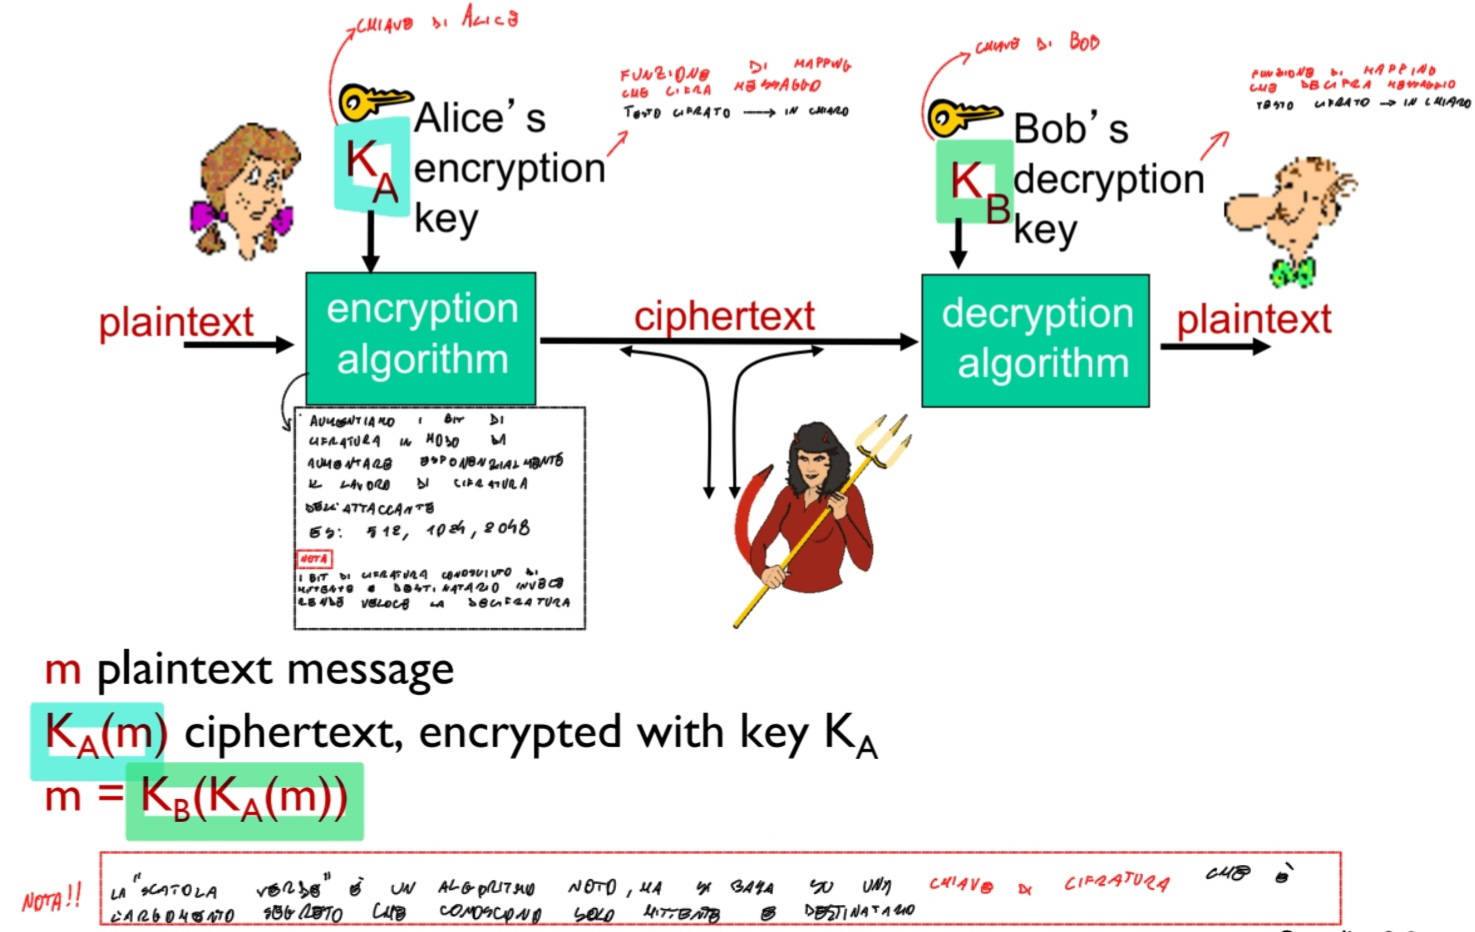
\includegraphics[width=1\textwidth]{immagini/crittorafia.jpg}
    \caption{Il linguaggio della crittografia: flusso da plaintext a ciphertext e viceversa.}
\end{figure}

\subsection{Rompere uno schema di cifratura (Crittanalisi)}

Un intruso (Trudy) può tentare di recuperare il messaggio originale o scoprire le chiavi. Esistono tre approcci principali di attacco :

\begin{notebox}{Tipologie di Attacco}
\begin{itemize}
    \item \textbf{Cipher-text only attack (Attacco al solo testo cifrato):}
    Trudy possiede solo il messaggio cifrato. Per decifrarlo può usare:
    \begin{itemize}
        \item \textit{Brute force:} Provare tutte le chiavi possibili.
        \item \textit{Analisi statistica:} Analizzare la frequenza dei caratteri nel testo cifrato.
    \end{itemize}
    
    \item \textbf{Known-plaintext attack (Attacco a testo in chiaro noto):}
    Trudy possiede sia il testo cifrato che il corrispondente testo in chiaro.

    
    \textit{Esempio:} In un cifrario monoalfabetico, questo permette di determinare le corrispondenze (es. 'a' $\rightarrow$ 'x').
    
    \item \textbf{Chosen-plaintext attack (Attacco a testo in chiaro scelto):}
    Trudy è in grado di ottenere il testo cifrato corrispondente a un testo in chiaro arbitrario scelto da lei. Questo è l'attacco più potente per dedurre lo schema o la chiave.
\end{itemize}
\end{notebox}

\subsection{Crittografia a Chiave Simmetrica}

% Placeholder Immagine: Crittografia Simmetrica
\begin{figure}[H]
    \centering
        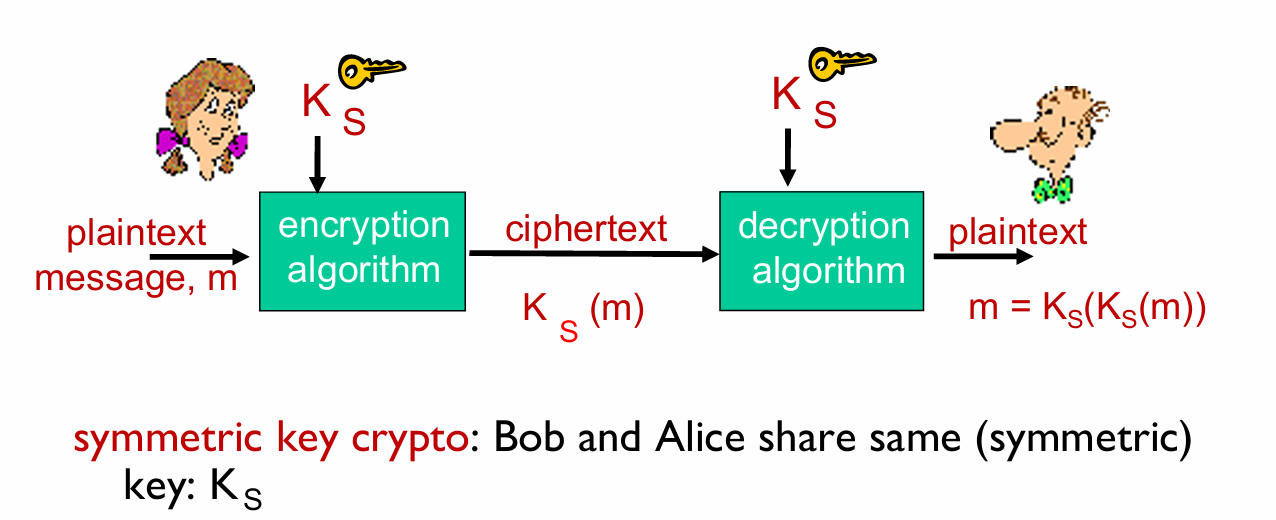
\includegraphics[width=0.8\linewidth]{immagini/Sym.png}
    \caption{Funzionamento della crittografia a chiave simmetrica.}
\end{figure}
In questo schema, Alice e Bob condividono la \textbf{stessa chiave segreta} ($K_S$) sia per cifrare che per decifrare ($K_A = K_B = K_S$).

\[ C = K_S(m) \quad \text{e} \quad m = K_S(C) \]

\subsection*{Esempi crittografia a chiave simmetrica}
\begin{itemize}
    \item \textbf{Cifrari a sostituzione:} Sostituiscono ogni elemento del testo in chiaro con un altro (es. Cifrario di Cesare, cifrari monoalfabetici). Sono vulnerabili all'analisi statistica.
    
\textit{Cifrario monoalfabetico:} ogni lettera viene sostituita con un'altra secondo una mappa fissa.

\begin{center}\ttfamily\small
\begin{tabular}{rl}
Testo in chiaro: & abcdefghijklmnopqrstuvwxyz \\
Chiave (cifrato): & mnbvcxzasdfghjklpoiuytrewq \\
\end{tabular}
\end{center}

\textbf{Esempio:} \texttt{bob. i love you. alice} $\to$ \texttt{nkn. s gktc wky. mgsbc}

Vulnerabile all'analisi delle frequenze. 

I \textit{cifrari polialfabetici} usano $n$ alfabeti in ciclo
(chiave = $n$ cifrari + pattern ciclico), rendendo l'analisi molto pi\`u difficile.
\newpage
    \item \textbf{DES (Data Encryption Standard):} Standard USA del 1993. Usa una chiave a 56 bit e blocchi a 64 bit. Oggi considerato insicuro (brute-forceable in meno di un giorno).

    esiste anche il TREDES che utilizza il DES tre volte di fila
    


    \begin{figure}[H]
        \centering
        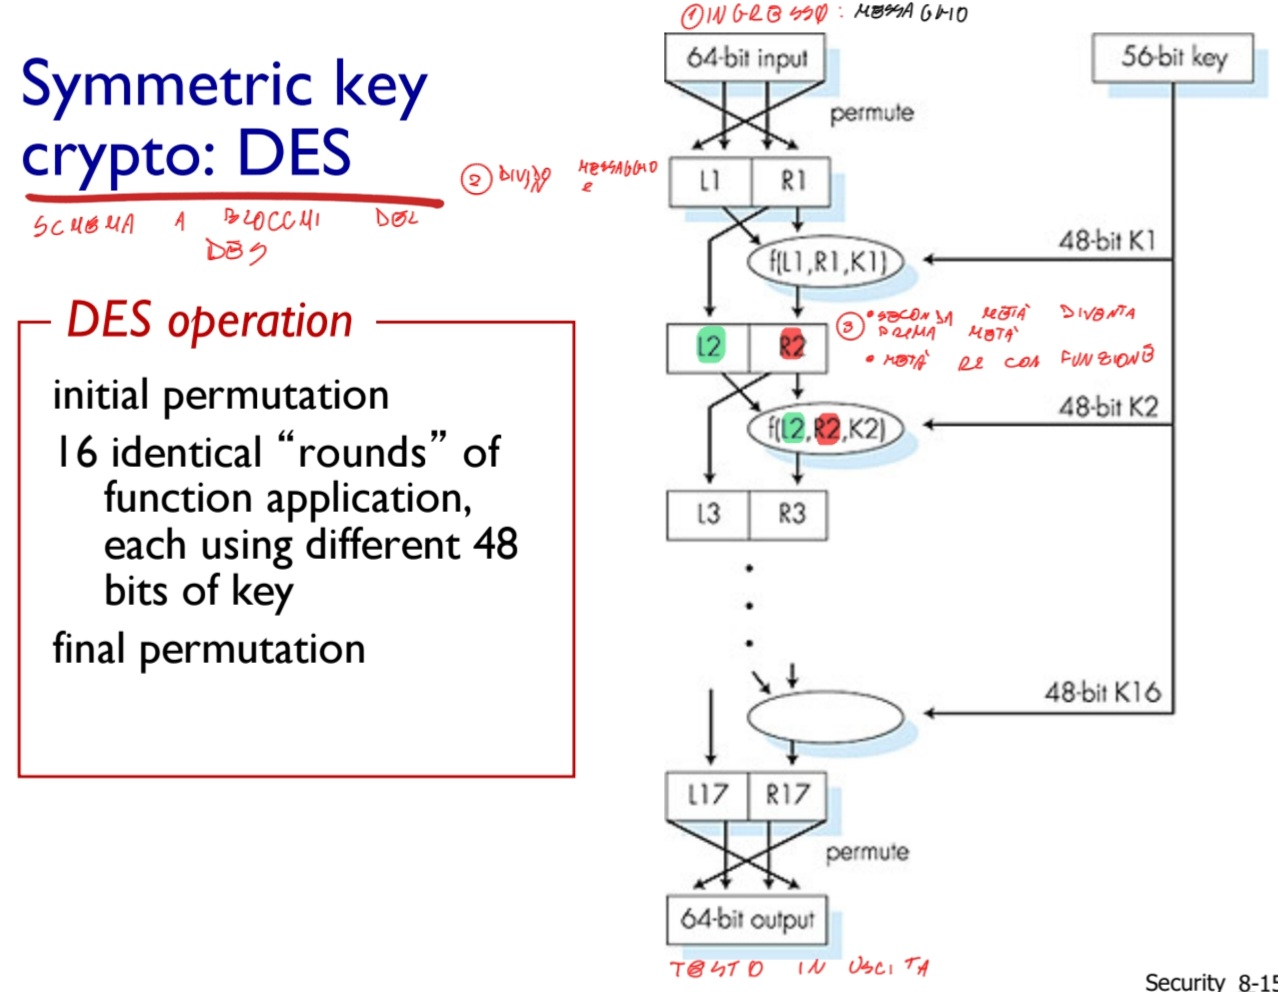
\includegraphics[width=0.8\linewidth]{immagini/DES.jpg}
        \caption{DES operazioni }
        \label{fig:placeholder}
    \end{figure}
    
    \item \textbf{AES (Advanced Encryption Standard):} Ha sostituito il DES nel 2001. Elabora i dati in blocchi da 128 bit e supporta chiavi di 128, 192 o 256 bit. È computazionalmente molto sicuro (richiederebbe miliardi di anni per essere rotto).
    
    Brute-force: 1 secondo su DES $\approx$ \textbf{149 trilioni di anni} su AES a 128 bit.
\end{itemize}




\newpage
\subsection{Crittografia a Chiave Pubblica}
Risolve il problema dello scambio delle chiavi tipico della crittografia simmetrica. Questo approccio, prevede che mittente e destinatario non condividano una chiave segreta. Ogni utente possiede invece una coppia di chiavi:
\begin{itemize}
    \item \textbf{Chiave Pubblica ($K^+$):} Nota a tutti, usata per cifrare.
    \item \textbf{Chiave Privata ($K^-$):} Nota solo al proprietario, usata per decifrare.
\end{itemize}

\begin{tcolorbox}[defbox,title=Propriet\`a fondamentali]
\begin{align*}
  \KBm\!\left(\KBp(m)\right) &= m \qquad \text{e} \qquad \KBp\!\left(\KBm(m)\right) = m \\
  &\text{Dato } \KBp\text{, \`e impossibile calcolare }\KBm.
\end{align*}
\end{tcolorbox}

\begin{notebox}{Prerequisito: Rappresentazione del Messaggio}
Nella crittografia RSA, un messaggio in chiaro è visto semplicemente come una sequenza di bit, che può essere univocamente rappresentata da un numero intero. Cifrare un messaggio equivale quindi a cifrare e trasformare quel numero.
\end{notebox}

\begin{defbox}{Algoritmo RSA (Rivest, Shamir, Adleman)}
L'algoritmo RSA si basa sulla difficoltà computazionale di fattorizzare grandi numeri interi. 
La generazione delle chiavi avviene in 5 passaggi:
\begin{enumerate}
    \item Si scelgono due grandi numeri \textbf{primi} $p$ e $q$ (es. di 1024 bit ciascuno).
    \item Si calcola 
    
    \begin{center}
        $n = p \cdot q$  e  $z = (p-1)(q-1) $  

        
        (z sarà composto da numeri pari, quindi il prodotto sarà pari)
    \end{center}}
    \newline
    
    \item Si sceglie un intero $e$ (con $e < n$) tale che non abbia fattori comuni 
    
    (divisori comuni )con $z$ ($e$ e $z$ sono "primi tra loro" ovvero con $\gcd(e,z)=1$.).
    \item Si calcola $d$ tale che $e \cdot d - 1$ sia esattamente divisibile per $z$ 
    
    (ovvero, $e \cdot d \pmod z = 1$).
    \item La \textbf{chiave pubblica} è $(n,e)$ e la \textbf{chiave privata} è $(n,d)$.
\end{enumerate}

\textbf{Operazioni di Cifratura e Decifratura:} \\
Per inviare un messaggio $m$ (dove $m < n$) a Bob, Alice calcola il testo cifrato $c$:
$$ c = m^e \mod n $$
Bob decifra il messaggio ricevuto calcolando:
$$ m = c^d \mod n $$
Tutto questo è reso possibile dall'aritmetica modulare, per cui avviene la "magia": $m = (m^e \mod n)^d \mod n$.
\end{defbox}


\begin{figure}[H]
    \centering
    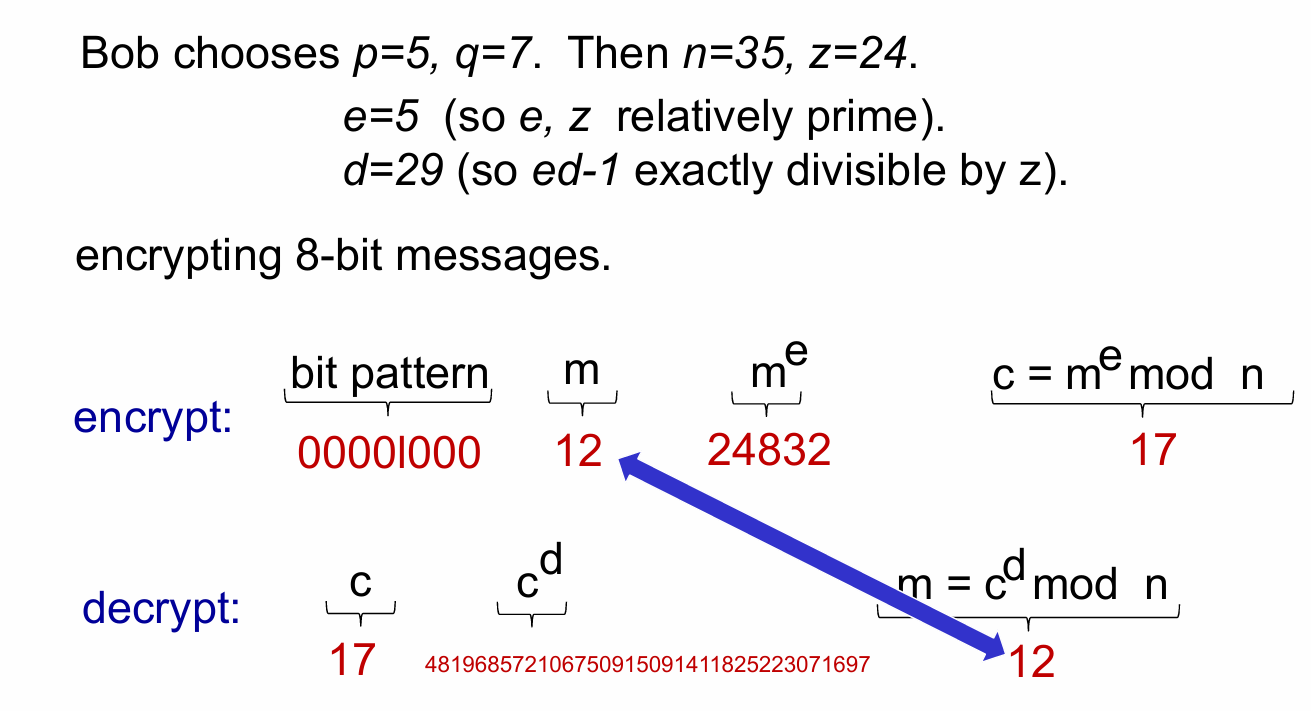
\includegraphics[width=0.8\linewidth]{immagini/RSA.png}
    \caption{Esempio RSA}
    \label{fig:placeholder}
\end{figure}
\begin{notebox}{Il Ruolo dei Bit di Padding}
Osservando la rappresentazione binaria del messaggio (es. \texttt{00001100} per il valore $m=12$), i bit iniziali aggiunti sono noti come bit di \textbf{padding}. Vengono inseriti per i seguenti motivi fondamentali:

\begin{enumerate}
    \item \textbf{Allineamento alla dimensione del blocco:} I sistemi crittografici operano su blocchi di dati di lunghezza fissa. Se il messaggio reale è più corto, è necessario "riempirlo" (padding) per fargli raggiungere la dimensione esatta richiesta dall'algoritmo.
    
    \item \textbf{Sicurezza e offuscamento semantico:}Il padding consiste in \textit{"informazioni messe per complicare l'interpretazione del messaggio"}. Nella sua forma base (\textit{Textbook RSA}), l'algoritmo è deterministico: cifrare due volte lo stesso messaggio produce lo stesso crittogramma. L'aggiunta di pattern di padding \textbf{randomizzati} garantisce che cifrando lo stesso messaggio si ottengano crittogrammi sempre diversi, neutralizzando gli attacchi statistici.
    
    \item \textbf{Segretezza e decodifica:} La struttura del padding viene concordata a priori (tramite standard appositi) e applicata \textbf{prima} della cifratura. L'intero blocco (padding + messaggio) diventa il numero $m$ che viene trasformato matematicamente. Trudy vede solo il crittogramma $c$ e non può sapere quali bit siano di padding senza decifrare il tutto. Solo il destinatario legittimo, applicando la chiave privata, decifra il blocco, riconosce le posizioni del padding, lo scarta e recupera il vero messaggio.
\end{enumerate}
\end{notebox}

\begin{notebox}{Proprietà RSA Fondamentale}
L'ordine di applicazione delle chiavi è invertibile. Questo è cruciale per le \textbf{Firme Digitali}:
$$ K_B^-(K_B^+(m)) = m = K_B^+(K_B^-(m)) $$
Usare prima la chiave pubblica e poi la privata porta allo stesso risultato dell'usare prima la privata e poi la pubblica.
\end{notebox}

\begin{urgentbox}{Limiti Pratici di RSA e Chiavi di Sessione}
\begin{itemize}
    \item \textbf{Sicurezza Computazionale:} La sicurezza di RSA si basa sull'ipotesi che fattorizzare il numero gigante $n$ per trovare $p$ e $q$ sia matematicamente troppo arduo. Ovvero è facile formulare una formula diretta ma arduo trovare quella inversa
    \item \textbf{Problema di Efficienza:} L'esponenziazione richiesta da RSA è computazionalmente molto intensiva. Algoritmi a chiave simmetrica come il DES (o AES) sono almeno 100 volte più veloci.
    \item \textbf{Soluzione (Session Keys):} Nella pratica, non si usa RSA per cifrare enormi flussi di dati. Si utilizza la crittografia a chiave pubblica solo per instaurare una connessione sicura iniziale, scambiandosi una \textbf{chiave simmetrica di sessione} ($K_S$). Una volta che entrambi possiedono $K_S$, la trasmissione dei dati prosegue usando la crittografia simmetrica (molto più rapida).
\end{itemize}
\end{urgentbox}

\begin{esempiobox}{La Pratica: Messaggi Corti vs Messaggi Lunghi (Crittografia Ibrida)}
Nella realtà operativa delle reti di calcolatori, la scelta di come applicare l'algoritmo RSA dipende drasticamente dalla mole di dati da trasmettere:

\begin{itemize}
    \item \textbf{Messaggi Corti:} Se il dato da proteggere è di dimensioni molto ridotte (ad esempio, un PIN, una password, un Nonce, o l'Hash di un documento per una firma digitale), l'algoritmo RSA può essere applicato \textit{direttamente} sull'intero contenuto. Il peso computazionale rimane gestibile e si garantisce la massima sicurezza senza passaggi intermedi.
    
    \item \textbf{Messaggi Lunghi (Approccio Ibrido):} Poiché RSA è computazionalmente oneroso, cifrare un'intera e-mail con allegati o un flusso video richiederebbe tempi inaccettabili. Si utilizza quindi l'efficienza della crittografia simmetrica combinata alla sicurezza dell'asimmetrica:
    \begin{enumerate}
        \item Alice genera una \textbf{chiave simmetrica di sessione} casuale ($K_S$), progettata per essere veloce ("usa e getta").
        \item Alice cifra l'intero blocco di dati $m$ usando la crittografia simmetrica (es. AES) con la chiave $K_S$.
        \item A questo punto, Alice usa RSA per cifrare \textit{esclusivamente} la chiave di sessione $K_S$, utilizzando la \textbf{chiave pubblica} di Bob ($K_B^+$).
        \item Alice trasmette a Bob il messaggio cifrato ($K_S(m)$) unito alla chiave di sessione cifrata ($K_B^+(K_S)$).
        \item Bob utilizza la propria \textbf{chiave privata} ($K_B^-$) per recuperare la chiave di sessione $K_S$. Una volta ottenuta, la applica per decifrare velocemente il corpo del messaggio.
    \end{enumerate}
\end{itemize}

Questo schema ibrido, alla base di protocolli come \textbf{SSL/TLS} e \textbf{IPsec}, permette di ottenere il meglio di entrambi i mondi: l'agilità di calcolo della crittografia simmetrica e la sicurezza nello scambio delle chiavi garantita dalla crittografia asimmetrica.
\end{esempiobox}




\newpage
\section{Autenticazione e Integrità del messaggio }

\subsection{Autenticazione degli End-Point}

\begin{notebox}{}
    L'obiettivo dell'autenticazione è permettere a Bob di accertarsi che Alice "dimostri" inequivocabilmente la propria identità. In una rete, tuttavia, Bob non può "vedere" fisicamente Alice. 
\end{notebox}


Vediamo l'evoluzione dei protocolli di autenticazione e i problemi che ognuno di essi cerca di risolvere:

\begin{itemize}
    \item \textbf{ap1.0:} Alice invia in chiaro il messaggio "Io sono Alice". 
    
    \textbf{Fallisce:} Trudy può semplicemente intercettare la comunicazione e dichiarare a sua volta di essere Alice.
    
    \item \textbf{ap2.0:} Alice invia il messaggio "Io sono Alice" in un pacchetto IP che contiene il suo indirizzo IP sorgente. 
    
    \textbf{Fallisce:} Trudy può creare un pacchetto falsificando l'indirizzo IP di Alice (\textit{IP spoofing}).
    
    \item \textbf{ap3.0:} Alice invia la sua password segreta in chiaro per "dimostrare" la sua identità. 
    
    \textbf{Fallisce:} Trudy può effettuare un \textit{playback/replay attack} , registrando il pacchetto di Alice e riproducendolo in seguito verso Bob per farsi autenticare.
    
    \item \textbf{ap3.1:} Alice invia la password segreta \textbf{cifrata}. 
    
    \textbf{Fallisce:} Anche se Trudy non conosce la password in chiaro, l'attacco di \textit{playback} funziona ancora, in quanto le basta registrare l'intero blocco cifrato e riutilizzarlo identico in seguito.
    
    \item \textbf{ap4.0 (Uso del Nonce e chiave simmetrica):} Per evitare l'attacco di playback/replay, si utilizza un \textbf{Nonce} ($R$), ovvero un numero usato \textit{una sola volta nella vita}. Bob invia $R$ ad Alice, la quale deve restituirlo cifrato con la chiave segreta condivisa ($K_{A-B}(R)$). Poiché solo Alice conosce la chiave ed è "viva" in quel momento, Bob ha la prova della sua identità. \\
    \textit{Limite:} Richiede che Alice e Bob condividano già una chiave simmetrica.
    
    \item \textbf{ap5.0 (Uso del Nonce e crittografia a chiave pubblica):} Svolge la stessa funzione del protocollo 4.0 ma utilizzando le tecniche a chiave pubblica per superare il problema dello scambio della chiave simmetrica. Bob invia il nonce $R$, e Alice lo restituisce cifrato con la propria \textbf{chiave privata} ($K_A^-(R)$). Bob verifica l'identità calcolando $K_A^+(K_A^-(R)) = R$ tramite la chiave pubblica di Alice.
\end{itemize}



\begin{center}
\begin{tabular}{lll}
\toprule
\textbf{Protocollo} & \textbf{Meccanismo} & \textbf{Fallimento} \\
\midrule
ap1.0 & Alice dichiara ``Sono Alice'' & Trudy fa lo stesso \\
ap2.0 & Alice include il suo IP & IP spoofing \\
ap3.0 & Alice include la password & Replay attack \\
ap3.1 & Alice cifra la password & Replay attack (il pacchetto cifrato viene ritrasmesso) \\
ap4.0 & Nonce + chiave simmetrica & Richiede chiave condivisa pre-esistente \\
ap5.0 & Nonce + chiave pubblica & Man-in-the-Middle (senza PKI) \\
\bottomrule
\end{tabular}
\end{center}

\begin{figure}[H]
    \centering
    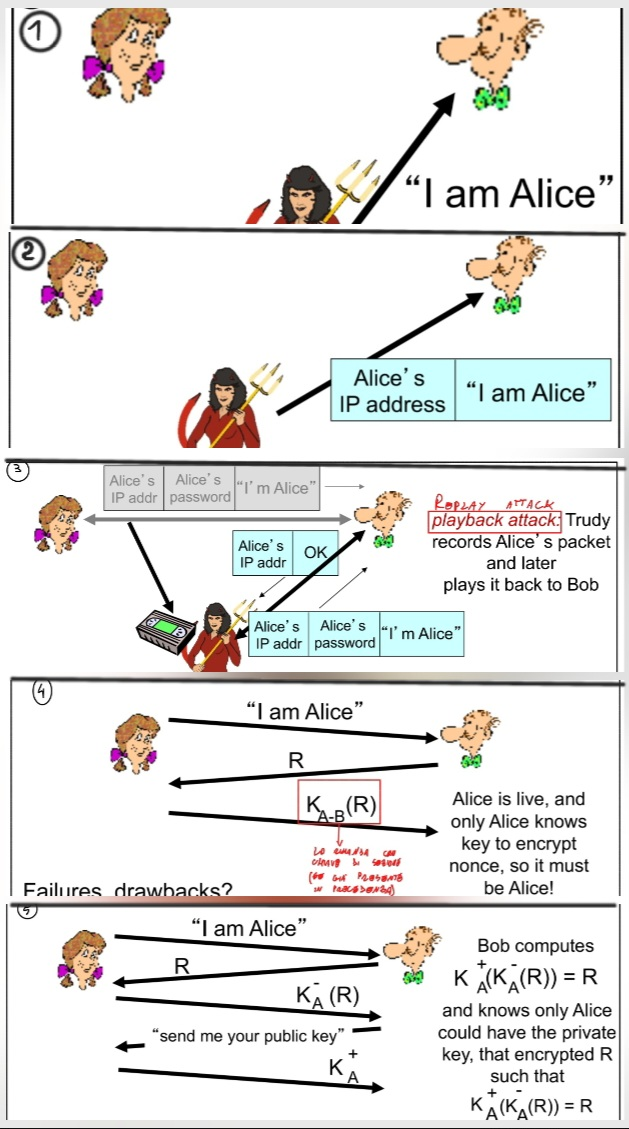
\includegraphics[width=0.7\linewidth]{immagini/autentic.jpg}
    \caption{Evoluzione dei protocolli di autenticazione e fallimenti associati.}
\end{figure}

\newpage
\begin{urgentbox}{La vulnerabilità di ap5.0: Man-in-the-Middle Attack}
Anche utilizzando crittografia a chiave pubblica e nonce, il protocollo ap5.0 presenta una grave falla di sicurezza se non c'è una certificazione delle chiavi.

Trudy si interpone tra Alice e Bob presentando la propria chiave pubblica
in luogo di quella altrui. Entrambi credono di comunicare direttamente:
\begin{enumerate}[noitemsep]
  \item Bob riceve $K_T^+$ (di Trudy) credendo sia $\KAp$.
  \item Alice riceve $K_T^+$ (di Trudy) credendo sia $\KBp$.
  \item Trudy decifra, legge/modifica e re-cifra tutto il traffico.
  \item Bob e Alice non si accorgono di nulla.
\end{enumerate}
\textbf{Soluzione:} infrastruttura a chiave pubblica (PKI) con Certification Authority.
\end{urgentbox}

\begin{figure}[H]
    \centering
    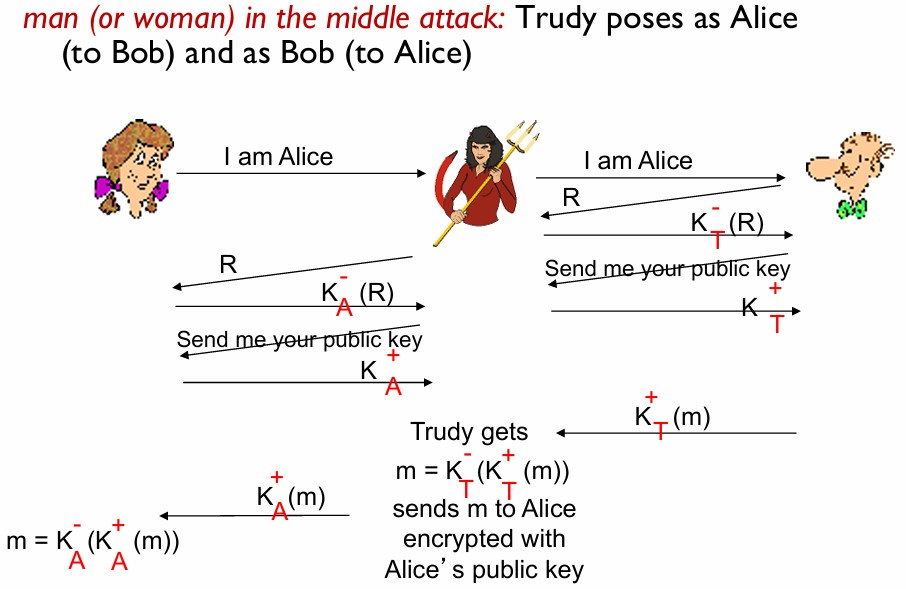
\includegraphics[width=0.8\linewidth]{immagini/Man_in_the_middle.jpg}
    \caption{Man in the middle, vengono sostituite le chiavi pubbliche e private con quelle dell'intruso che può modificare i messaggi a suo piacimento }
\end{figure}

\begin{notebox}{}
     Il problema è lo \textbf{scambio di chiavi} in cui non siamo sicuri della chiave pubblica che ci viene fornita per cifrare il messaggio. E' necessario quindi avere dei certificati di sicurezza che garantisce quale sia la nostra chiave pubblica.
Tali certificati sono prodotti da servizi terzi in rete dette \hyperref[subsec:cert-chiavi]{Certification Authority (CA)} multiple (pag 17).
\end{notebox}


\newpage
\subsection{Integrità e Hash (Message Digest)}
Dobbiamo anche garantire che il messaggio non venga modificato da un intruso (integrità),oltre ad essere sicuri della persona che ce lo manda(provenienza,come visto nel paragrafo precedente)
Modificando anche un solo bit il messaggio mandato sarà completamnete illeggibile.

Poiché la crittografia a chiave pubblica(RSA) è computazionalmente pesante, non viene quasi mai usata per cifrare interi messaggi lunghi. Per garantire l'integrità dei dati si usa un'impronta digitale di lunghezza fissa, estremamente veloce da calcolare: il \textbf{Message Digest} (consiste nella trasformazione dell'intero messaggio m in un messaggio H(m) più piccolo ottenuto tramite funzione di Hash).

\begin{esempiobox}{funzione di hash}
    Prendiamo un dominio \textbf{infinito} formato da m -> funzuine f che prende oggetti dal domio -> elementi mappati tramite la funzione f in un codominio \textbf{finito}
\end{esempiobox}

\begin{defbox}{Proprietà della Funzione di Hash $H(m)$}
Una funzione crittografica di Hash trasforma un messaggio $m$ di lunghezza arbitraria in un output $H(m)$ di lunghezza \textbf{fissa} (chiamate fingerprint che appartengono al codominio finito). Affinché sia considerata sicura, deve garantire:
\begin{itemize}
    \item \textbf{Unidirezionalità (One-way):} Dato un digest $x$, deve essere computazionalmente impossibile risalire al messaggio originale $m$ tale che $x = H(m)$.
    \item \textbf{Resistenza alle collisioni:} È computazionalmente impossibile trovare due messaggi diversi $x$ e $y$ tali che $H(x) = H(y)$. E' praticamente impossibile trovare messaggi divesri che vengono mappati nello stesso elemento. Questo perchè randomizza la mappatura degli elementi
    \item\textbf{Distanza dei risultati} anche messaggi molto vicini inizialmente possono essere mappati in messaggi molto distanti tra loro nel codominio finito di arrivo
\end{itemize}
\end{defbox}

\begin{notebox}{Algoritmi Comuni e Controesempi}
\begin{itemize}
    \item \textbf{MD5:} Produce un digest a 128 bit (RFC 1321).
    \item \textbf{SHA-1:} Produce un digest a 160 bit (Standard US NIST). 
    \item \textit{Attenzione:} Il classico \textbf{Internet Checksum} a 16 bit (es. quello usato nell'header IPv4) \textbf{non} è una funzione crittografica sicura! È matematicamente banale trovare due messaggi diversi che generino la stessa identica somma (ad esempio tramite proprietà commutativa). E' many-to-one ma NON \`e resistente alle
collisioni $\to$ non adatto per sicurezza. 
\end{itemize}
\end{notebox}

\newpage
\subsection{Firma Digitale (Digital Signature)}
La firma digitale è l'equivalente crittografico della firma autografa. È verificabile, non falsificabile e dimostra in modo inconfutabile l'identità del creatore. 
Nella pratica, per questioni di efficienza, \textbf{non si firma mai l'intero documento, ma solo il suo Hash}.

\begin{esempiobox}{Processo di Firma e Verifica}
\textbf{1. Firma (Mittente - Bob):}
\begin{itemize}
    \item Bob calcola l'hash del messaggio in chiaro: $H(m)$.
    \item Bob cifra il digest appena ottenuto con la propria \textbf{chiave privata} ($K_B^-$). Il risultato, $K_B^-(H(m))$, è la vera e propria firma digitale.
    \item Bob invia ad Alice il messaggio in chiaro $m$ unito alla firma digitale.
\end{itemize}

\textbf{2. Verifica (Destinatario - Alice):}
\begin{itemize}
    \item Alice riceve $m$ e la firma. Calcola a sua volta l'hash del messaggio in chiaro ricevuto: $H(m)$.
    \item Alice decifra la firma usando la \textbf{chiave pubblica} di Bob ($K_B^+$).
    \item Se l'hash calcolato da Alice \textbf{coincide esattamente} con l'hash decifrato, la firma è valida.
\end{itemize}
\end{esempiobox}


Schema completo: Bob calcola l'hash del messaggio e cifra l'hash con la sua chiave privata.

\begin{center}
\begin{tikzpicture}[
  box/.style={draw=uniboblue,fill=unibolight,rounded corners=3pt,
    minimum width=2.4cm,minimum height=0.7cm,font=\small,align=center},
  arr/.style={-Latex,thick,draw=uniboblue!80}]
  %% Bob
  \node[box](mb){$m$};
  \node[box,right=0.9cm of mb](hb){$H(\cdot)$};
  \node[box,right=0.9cm of hb](eb){Cifra $\KBm$};
  \node[box,right=0.9cm of eb](sb){firma $=\!\KBm\!(H(m))$};
  \node[above=0.15cm of mb,font=\small\bfseries\color{uniboblue}]{Bob (firma):};
  \draw[arr](mb)--(hb);\draw[arr](hb)--(eb);\draw[arr](eb)--(sb);
  %% separator
  \draw[dashed,gray!60]($(mb.south west)+(-0.1,-0.5)$)--($(sb.south east)+(0.1,-0.5)$);
  %% Alice
  \node[box,below=1.4cm of mb](ma){$m$};
  \node[box,right=0.9cm of ma](ha){$H(\cdot)$};
  \node[box,below=1.4cm of sb](da){Decifra $\KBp$};
  \node[box,right=0.9cm of ha,draw=okgreen,fill=green!8](eq){Uguale?};
  \node[above=0.15cm of ma,font=\small\bfseries\color{uniboblue}]{Alice (verifica):};
  \draw[arr](ma)--(ha);\draw[arr](ha.east)--(eq.west);
  \draw[arr](da.west)--(eq.east);
  \draw[arr,dashed](mb.south)--(ma.north);
  \draw[arr,dashed](sb.south)--(da.north);
\end{tikzpicture}
\end{center}

\begin{figure}[H]
    \centering
    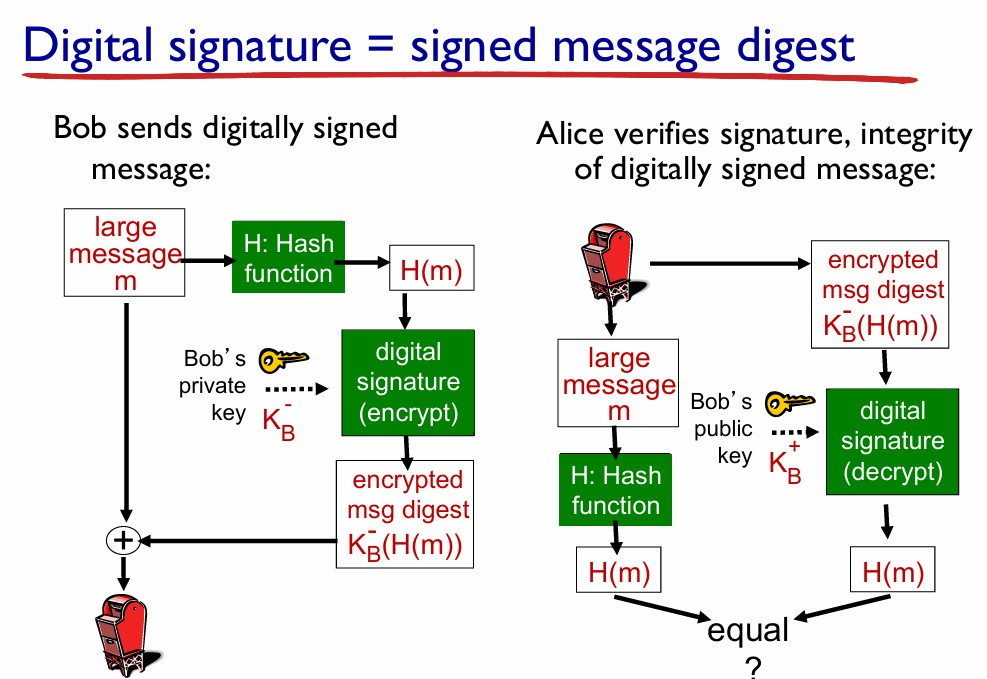
\includegraphics[width=0.8\linewidth]{immagini/digital_signature.jpg}
    \caption{ BOB: Manda m in chiaro direttamente nella mail e poi calcola l'hash e firma digitalmente il messaggio ridotto (lo manda in una busta privata firmata da lui).
    Alice: calcola H(m) del messaggio ricevuto da BoB e lo confronta con quello chiuso da Bob ed inviato nella mail}
\end{figure}

Le garanzie definitive fornite dalla Firma Digitale (combinata all'Hash) sono:
\begin{itemize}
    \item \textbf{Autenticazione dell'origine:} Solo Bob possiede la chiave privata necessaria per generare quella specifica firma.
    \item \textbf{Integrità del messaggio:} Se Trudy altera $m$ durante il transito, l'hash ricalcolato da Alice sarà diverso da quello contenuto nella firma decifrata, facendo fallire il controllo  (facendosi che il pacchetto venga buttato).
    \item \textbf{Non ripudio:} Alice può usare il messaggio e la firma come prova inconfutabile (ad es. "in tribunale") per dimostrare che Bob lo ha effettivamente firmato.
\end{itemize}


\newpage
\subsection{Certificazione delle Chiavi Pubbliche
(CA)}
\label{subsec:cert-chiavi}
Per risolvere definitivamente il problema del Man-in-the-Middle(ap5.0,di pag 13) e dello scambio sicuro delle chiavi, si introduce il concetto di \textbf{Certification Authority (CA), la quale lega la chiave pubblica all'identit\`a del titolare}.

\begin{esempiobox}{La motivazione: Lo "Scherzo della Pizza" }
Per capire perché la sola crittografia a chiave pubblica non basta, immaginiamo che Trudy voglia fare uno scherzo a Bob.
\begin{itemize}
    \item Trudy crea un finto ordine via e-mail: \textit{"Cara Pizzeria, per favore consegnami 4 pizze ai peperoni. Grazie, Bob"}.
    \item Trudy firma l'ordine cifrando l'hash con la \textbf{propria} chiave privata.
    \item Trudy invia l'ordine alla pizzeria.
    \item Insieme all'ordine, Trudy invia alla pizzeria la \textbf{propria} chiave pubblica, dichiarando però che si tratti della chiave pubblica di Bob.
    \item La pizzeria usa la chiave ricevuta per verificare la firma. Poiché la chiave è effettivamente quella di Trudy, la decodifica ha successo. La pizzeria crede ciecamente all'identità dichiarata e consegna le pizze (che lui odia) a Bob.
\end{itemize}
\textbf{Il problema:} La pizzeria non ha alcun modo per accertarsi che la chiave pubblica ricevuta appartenga realmente a Bob.
\end{esempiobox}

\begin{defbox}{Certification Authority (CA)}
Una CA è un'entità fidata (istituzionale o commerciale) che si occupa di vincolare (bind) una chiave pubblica a una specifica entità $E$ (una persona, un server, un router).
    
\textbf{1. Registrazione (Creazione del Certificato):}
\begin{itemize}
    \item L'entità $E$ registra la propria chiave pubblica presso la CA.
    \item $E$ deve fornire una "prova di identità" (es. documenti fisici o verifiche del dominio).
    \item La CA crea un \textbf{Certificato} che unisce le informazioni identificative di $E$ alla sua chiave pubblica.
    \item La CA \textbf{firma digitalmente} questo certificato cifrandone l'hash con la \textit{propria} chiave privata ($K_{CA}^-$). Questo equivale a dire: "La CA certifica che questa è la vera chiave di E".
\end{itemize}
    
\textbf{2. Utilizzo e Verifica:} \\
Quando Alice vuole comunicare in modo sicuro con Bob e le serve la sua chiave pubblica:
\begin{itemize}
    \item Alice ottiene il certificato di Bob (inviatole da Bob stesso o scaricato da una directory pubblica).
    \item Alice applica la \textbf{chiave pubblica della CA} ($K_{CA}^+$) (che è preinstallata in modo sicuro nel suo sistema operativo o browser) per decifrare la firma sul certificato di Bob.
    \item Se la verifica ha successo, Alice estrae la chiave pubblica di Bob ($K_B^+$) dal certificato, avendo la certezza assoluta che sia autentica e non appartenga a Trudy.
\end{itemize}
\end{defbox}

% Placeholder Immagine: Processo di certificazione CA e verifica

\begin{figure}[H]
    \centering
    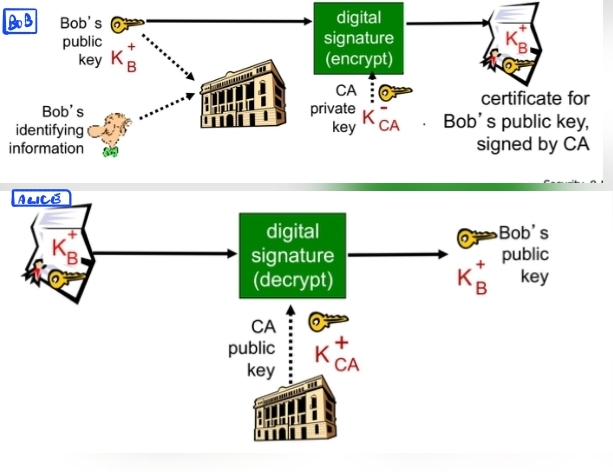
\includegraphics[width=0.6 \linewidth]{immagini/autenticate.jpg}
    \caption{Processo di creazione e verifica di un certificato digitale tramite CA.
     La CA firma la chiave pubblica di Bob con la propria chiave privata, Alice la verifica con la chiave pubblica della CA}
\end{figure}


\begin{notebox}{Ruolo delle CA contro il Man-in-the-Middle e Scadenza}
Le Certification Authorities (CA) sono la contromisura definitiva contro gli attacchi Man-in-the-Middle (MitM) grazie a due meccanismi fondamentali:

\begin{itemize}
    \item \textbf{Neutralizzazione del MitM:} Se Trudy tenta di intercettare la comunicazione e inviare ad Alice la \textit{propria} chiave pubblica spacciandola per quella di Bob, fallirà. Trudy non possiede la chiave privata della CA, quindi non può generare una firma digitale valida per il finto certificato. Quando Alice verifica la firma con la chiave pubblica della CA (già verificata e preinstallata nel suo sistema operativo o browser), la contraffazione viene immediatamente smascherata e la connessione rifiutata.
    
    \item \textbf{Scadenza Temporale:} La fiducia crittografica non è mai eterna. Ogni certificato emesso da una CA ha un periodo di validità ben definito (con una data di inizio e una \textbf{data di scadenza}). Questo limita temporalmente i danni nel caso in cui una chiave privata venga scoperta.
    
    \item \textbf{Revoca (CRL):} Se la chiave privata di Bob viene compromessa o rubata \textit{prima} della naturale scadenza del certificato, la CA ha il compito di invalidarlo attivamente inserendolo in una \textbf{CRL} (\textit{Certificate Revocation List}). I client (come i browser) controllano questa lista per assicurarsi che il certificato, anche se non ancora scaduto, sia ancora considerato affidabile.
\end{itemize}
\end{notebox}
\newpage


\subsection{Ruoli della Firma digitale e della CA}
\begin{urgentbox}{Autenticazione mittente e integrità messaggio}
    Ecco come si dividono i compiti nella crittografia moderna:

\begin{itemize}
    \item \textbf{Il ruolo della CA (Autenticazione dell'entità):} Garantisce in modo assoluto che la chiave pubblica di Bob ($K_B^+$) appartenga veramente a Bob e non a Trudy. Il lavoro della CA finisce sostanzialmente qui.
    
    \item \textbf{Il ruolo della Firma Digitale (Integrità e Non Ripudio):} Per garantire che il messaggio specifico non sia stato alterato (che Trudy non abbia cambiato ``4 pizze margherita'' in ``4 pizze ai peperoni''), si usa la Firma Digitale basata su funzioni di Hash.
\end{itemize}
\end{urgentbox}


\newpage
\section{Sicurezza delle E-mail}

Progettare un sistema di e-mail sicuro significa dover garantire tre proprietà fondamentali:
\begin{itemize}
    \item Confidenzialità
    \item Autenticazione del mittente 
    \item Integrità del messaggio. 
\end{itemize}Vediamo come queste proprietà possono essere implementate progressivamente.

\subsection{Scenario 1: Solo  Confidenzialità (Riservatezza)}
In questo scenario, Alice vuole inviare un'e-mail a Bob assicurandosi che solo lui possa leggerla, ma non si preoccupa di dimostrare la propria identità. Poiché cifrare un intero messaggio con RSA è troppo lento, si usa un approccio ibrido.

\begin{itemize}
    \item \textbf{Fase di Cifratura (Alice):} 
    
\begin{enumerate}[noitemsep]
  \item Genera una chiave simmetrica casuale $K_S$.
  \item Cifra il messaggio con $K_S$: $K_S(m)$ (veloce).
  \item Cifra $K_S$ con la chiave pubblica di Bob: $\KBp(K_S)$.
  \item Invia: $\bigl\{K_S(m),\;\KBp(K_S)\bigr\}$.
\end{enumerate}
    \item \textbf{Fase di Decifratura (Bob):} Bob usa la propria \textbf{chiave privata} ($K_B^-$) per decifrare e recuperare $K_S$. Una volta ottenuta, usa $K_S$ per decifrare il messaggio,ovvero  usa $K_S$ su $K_S(m)$.
\end{itemize}

\begin{urgentbox}{Limite dello Scenario 1: Nessuna Garanzia sul Mittente}
Poiché la chiave pubblica di Bob è nota a tutti, Trudy (o chiunque altro) potrebbe generare una propria chiave di sessione $K_S$, cifrare un messaggio falso e inviarlo a Bob fingendo di essere Alice. Bob riuscirà a leggere il messaggio in modo confidenziale, ma non ha alcun modo per accertarsi di chi sia il reale mittente.
\end{urgentbox}

% Placeholder Immagine: Confidenzialità
\begin{figure}[H]
    \centering
    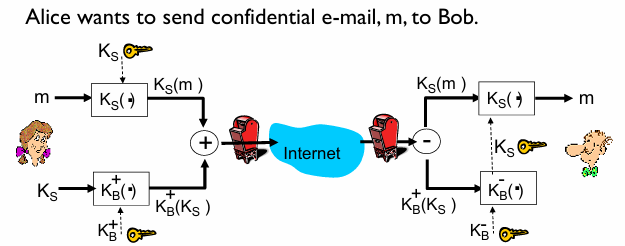
\includegraphics[width=0.8 \linewidth]{immagini/confident.png}
    \caption{Invio di un'e-mail garantendo solo la confidenzialità (approccio ibrido).}
\end{figure}

\newpage
\subsection{Scenario 2: Autenticazione e Integrità(non modificato / non ripudio) (senza Confidenzialità)}
In questo caso, Alice vuole che Bob sia assolutamente certo che il messaggio provenga da lei e non sia stato alterato. Si utilizza la Firma Digitale.

\begin{itemize}
    \item \textbf{Invio (Alice):} Alice calcola l'hash del messaggio $H(m)$ e lo cifra con la propria \textbf{chiave privata} ($K_A^-$), creando la firma digitale.
    
    Invia a Bob il messaggio \textbf{in chiaro} unito alla firma 
\[ \quad m \quad \text{e} \quad \KAm\!\bigl(H(m)\bigr)
\].
    \item \textbf{Verifica (Bob):} Bob riceve il pacchetto. Separa il messaggio dalla firma. Calcola autonomamente l'hash di $m$. Poi decifra la firma usando la \textbf{chiave pubblica di Alice} ($K_A^+$). Se i due hash coincidono, il messaggio è integro e autentico.
\end{itemize}

\begin{urgentbox}{Limite dello Scenario 2: Messaggio non Segreto}
In questo scenario, la crittografia viene applicata solamente all'Hash per creare la firma. Il corpo del messaggio $m$ viaggia in chiaro attraverso la rete. Se Trudy intercetta il pacchetto, non può modificarlo senza essere scoperta, ma può leggerne perfettamente tutto il contenuto, annullando la segretezza della comunicazione.
\end{urgentbox}

% Placeholder Immagine: Autenticazione e Integrità
\begin{figure}[H]
    \centering
     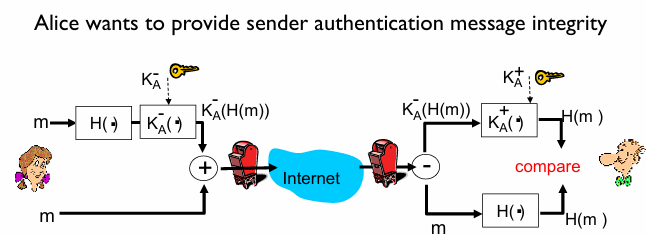
\includegraphics[width=0.8 \linewidth]{immagini/hash.png}
    \caption{Invio di un'e-mail garantendo autenticazione e integrità tramite firma digitale.}
\end{figure}

\newpage

\subsection{Scenario 3: Confidenzialità(Riservatezza) e Integrità (senza Autenticazione dell'origine)}
Un quesito d'esame classico riguarda l'omissione della firma digitale pur mantenendo l'hash. In questo scenario, Alice vuole che il messaggio sia segreto e che Bob possa verificare che non ci siano stati errori di trasmissione, ma decide di non firmarlo con la sua chiave privata.

\begin{itemize}
    \item \textbf{Invio (Alice):} Alice calcola l'hash del messaggio $H(m)$ e lo concatena direttamente al messaggio in chiaro. Poi cifra tutto il blocco con una chiave di sessione $K_S$. Infine, cifra $K_S$ con la chiave pubblica di Bob.
    
    \begin{center}
        Invia: $\bigl\{K_S\bigl(m \parallel H(m)\bigr),\;\KBp(K_S)\bigr\}$
    \end{center}
    
    \item \textbf{Verifica (Bob):} Bob usa la sua $\KBm$ per ricavare $K_S$. Decifra il blocco, separa $m$ da $H(m)$, ricalcola l'hash di $m$ e verifica che coincida.
\end{itemize}

\begin{urgentbox}{La vulnerabilità dello Scenario 3 (Il Trabocchetto)}
Se l'hash ricalcolato da Bob coincide, egli ha la garanzia assoluta dell'**Integrità del transito** (il messaggio non è stato corrotto da disturbi di linea o alterato al volo da un router). \textbf{Tuttavia, NON ha alcuna garanzia sul mittente}.

Trudy potrebbe scrivere un finto messaggio $m'$, calcolarne l'hash $H(m')$, cifrare il tutto con una \textit{sua} chiave $K_{S2}$ e inviare il pacchetto a Bob cifrando $K_{S2}$ con $\KBp$. Bob decifrerà tutto correttamente, gli hash coincideranno, ma il messaggio proverrà dall'attaccante. Senza la crittografia asimmetrica applicata all'hash (la firma con la chiave privata), l'autenticazione cade.
\end{urgentbox}

\newpage
\subsection{Scenario 4: Sicurezza Completa (Il pacchetto completo)}
Per ottenere un'e-mail totalmente sicura, Alice deve combinare i due scenari precedenti. Questo è l'approccio standard utilizzato da protocolli come PGP (Pretty Good Privacy).

\begin{esempiobox}{Processo di invio con Sicurezza Completa}
Alice vuole garantire Riservatezza, Autenticazione e Integrità. Per farlo, deve utilizzare contemporaneamente \textbf{tre chiavi diverse} (la propria privata $\KAm$ , la pubblica di Bob  $\KBp$ e una simmetrica nuova $K_S$).

\begin{enumerate}
    \item \textbf{Firma (Autenticazione/Integrità):} Alice calcola l'hash del messaggio $H(m)$ e lo cifra con la sua \textbf{chiave privata} ($K_A^-$) garantisce che sia stata solo alice a scrivere  il messaggio,ovvero che sia autentico 
    
    \textbf{NOTA}: (l'utilizzo di $K_{A}^-$ viene fatto solo all'invio del primo messaggio, a seguire si usa solo chiave simmetrica pre criptare l'hash).

    \begin{center}
         Calcola firma: $s = \KAm\!\bigl(H(m)\bigr)$.
    \end{center}

    \item Concatena questa firma digitale al messaggio originale $m$.
\begin{center}
    Concatena: $P = m \| s$.
\end{center}
    \vspace{0.5cm}

    
    \item \textbf{Cifratura del Corpo (Confidenzialità):} Alice genera una chiave simmetrica di sessione ($K_S$) . Cifra l'intero blocco (Messaggio + Firma) utilizzando $K_S$.

    \begin{center}
        Cifra con $K_S$: $K_S(P)$.
    \end{center}
    \item \textbf{Cifratura della Chiave:} Alice cifra la chiave di sessione $K_S$ utilizzando la \textbf{chiave pubblica di Bob} ($K_B^+$).

    \begin{center}
        Cifra $K_S$: $\KBp(K_S)$.
    \end{center}
    \item \textbf{Invio:} Alice spedisce su Internet il pacchetto cifrato e la chiave di sessione cifrata.

    \begin{center}
        Invia: $\bigl\{K_S(P),\;\KBp(K_S)\bigr\}$.
    \end{center}
\end{enumerate}


Quando Bob riceve i dati, compie le operazioni inverse: usa la sua chiave privata per ottenere $K_S$, usa $K_S$ per decifrare il blocco, e infine usa la chiave pubblica di Alice per verificare la firma digitale sull'hash.
\end{esempiobox}




% Placeholder Immagine: Sicurezza Completa
\begin{figure}[H]
    \centering
     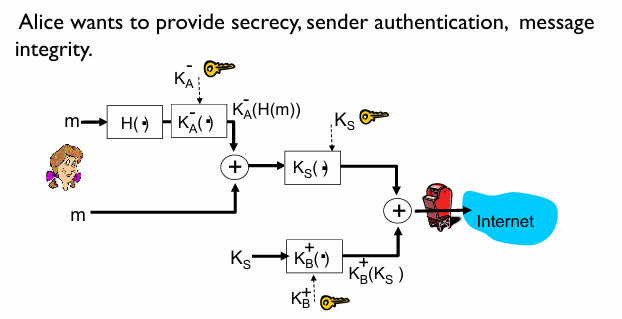
\includegraphics[width=0.5\linewidth]{immagini/completo.png}
    \caption{Schema completo per l'e-mail sicura: Confidenzialità, Autenticazione e Integrità.}
\end{figure}


\subsection{Scenario 4bis: Sicurezza Completa (Con anche nonce)}
\begin{notebox}{\textbf{Il Nonce: Protezione contro il Replay Attack}}
Nonostante lo \textbf{Scenario 4} (Sicurezza Completa) garantisca riservatezza, integrità e autenticità, esiste ancora una vulnerabilità: l'\textbf{attacco di Replay}. Trudy, pur non potendo leggere o modificare il messaggio, potrebbe catturare il pacchetto cifrato e rispedirlo identico più volte (ad esempio, un ordine di bonifico).

Per risolvere questo problema si introduce il \textbf{Nonce} (\textit{Number used ONCE}):
\begin{itemize}[leftmargin=*]
    \item \textbf{Definizione:} Un numero casuale o un identificativo univoco che viene utilizzato una sola volta per ogni sessione o messaggio.
    \item \textbf{Funzionamento:} Il mittente inserisce il Nonce all'interno del messaggio prima  cifrarlo. Il destinatario memorizza i Nonce ricevuti recentemente.
    \item \textbf{Verifica della "Freschezza":} Se il destinatario riceve un messaggio con un Nonce già visto o non valido, lo scarta immediatamente, classificandolo come un tentativo di duplicazione (Replay).
\end{itemize}

\textbf{Alternativa per le E-mail:} Poiché nelle comunicazioni asincrone (come la posta elettronica) non è sempre possibile scambiare un Nonce in tempo reale, si utilizza spesso un \textbf{Timestamp} (marca temporale) all'interno del pacchetto cifrato per garantirne la validità temporale.
\end{notebox}

\newpage
\begin{esempiobox}{Formulazione Sicurezza Completa con Nonce}
Per integrare la protezione contro il Replay Attack, Alice deve includere il Nonce (indichiamolo con $R$) inviatogli da BOB,  \textbf{prima} di calcolare l'hash e firmare il messaggio.

In questo modo, l'identificativo temporale è protetto sia dall'alterazione (tramite firma) sia dall'intercettazione (tramite cifratura).

Ecco come cambiano i passaggi visti nello Scenario 4:

\begin{enumerate}
\item Bob invia un nonce ad Alice
       
    \item \textbf{Firma (Autenticazione/Integrità) e integrazione del Nonce:} Alice calcola l'hash del messaggio, accoda il Nonce R  e lo cifra con la sua chiave privata ($\KAm$).
    \begin{center}
        Calcola firma: $s = \KAm\!\bigl(H(m) || R\bigr)$
    \end{center}
    
    \item \textbf{Composizione del blocco:} Concatena il messaggio originale, il Nonce e la firma.
    \begin{center}
        Concatena: $P = m  \parallel s$
    \end{center}
    
    \item \textbf{Cifratura (Confidenzialità):} Alice genera la chiave di sessione $K_S$ e cifra l'intero blocco $P$. Poi cifra $K_S$ con la chiave pubblica di Bob ($\KBp$).
    \begin{center}
        Dati cifrati: $K_S(P) = K_S\Bigl(m  \parallel \KAm\!\bigl(H(m )\parallel R\bigr)\Bigr)$ \\
        Chiave cifrata: $\KBp(K_S)$
    \end{center}
    
    \item \textbf{Invio del pacchetto finale:}
    \begin{center}
        Invia: $\bigl\{K_S\Bigl(m \parallel \KAm\!\bigl(H(m )\parallel R\bigr)\Bigr),\;\KBp(K_S)\bigr\}$
    \end{center}
\end{enumerate}


\textbf{Verifica di Bob:} Quando Bob riceve e decifra il blocco, estrae $R$. Se $R$ è un numero di sequenza diverso da quello inviato inizialmente Bob scarta l'intero pacchetto identificandolo come un Replay Attack.
\end{esempiobox}

\begin{figure}[H]
    \centering
    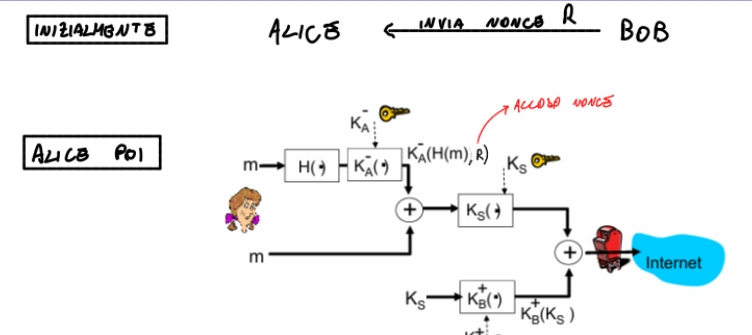
\includegraphics[width=0.9\linewidth]{immagini/SICTOT.jpg}
    \caption{}
    \label{fig:placeholder}
\end{figure}


\newpage
\subsection{Tabella Riassuntiva per Esercizi (Combinazioni E-mail)}

Questa tabella è uno strumento essenziale per risolvere gli esercizi di progettazione. Spesso viene richiesto di individuare "quali proprietà sono garantite" da un determinato pacchetto, o "quali chiavi" deve usare Alice per ottenere un certo livello di sicurezza.

\begin{center}
\renewcommand{\arraystretch}{1.5}
\small
\begin{tabularx}{\textwidth}{|>{\columncolor{unibolight}\bfseries}p{3.5cm}|X|p{2.5cm}|p{2.5cm}|p{2.5cm}|}
\hline
\rowcolor{uniboblue} 
\textcolor{white}{\textbf{Obiettivo di Sicurezza}} & 
\textcolor{white}{\textbf{Formato del Pacchetto Trasmesso}} & 
\textcolor{white}{\textbf{Chiavi usate da Alice}} & 
\textcolor{white}{\textbf{Chiavi usate da Bob}} & 
\textcolor{white}{\textbf{Vulnerabilità Principale}} \\
\hline

Solo Confidenzialità & 
$K_S(m)$ unito a $\KBp(K_S)$ & 
$K_S$, $\KBp$ & 
$\KBm$ & 
Chiunque può falsificare il mittente (No Autenticazione). \\
\hline

Autenticazione + Integrità (Firma Digitale) & 
$m$ unito a $\KAm\bigl(H(m)\bigr)$ & 
$\KAm$ & 
$\KAp$ & 
Il messaggio viaggia in chiaro (No confidenzialità). \\
\hline

Confidenzialità + Integrità & 
$K_S\bigl(m \parallel H(m)\bigr)$ unito a $\KBp(K_S)$ & 
$K_S$, $\KBp$ & 
$\KBm$ & 
Chiunque può creare un pacchetto valido (No Autenticazione). \\
\hline

\textbf{Sicurezza Completa} (Sign-then-Encrypt) & 
$K_S\Bigl(m \parallel \KAm\bigl(H(m)\bigr)\Bigr)$ unito a $\KBp(K_S)$ & 
$K_S$, $\KBp$, $\KAm$(solo al primo invio) & 
$\KBm$, $\KAp$ & 
Soggetto a \textit{Replay Attack} se non si usa un Nonce/Timestamp. \\
\hline
\end{tabularx}
\end{center}

\vspace{0.4cm}
\begin{esempiobox}{Dritte pratiche per l'esame}
\begin{itemize}
    \item \textbf{La regola d'oro per le chiavi:}
    \begin{itemize}
        \item \textbf{CONFIDENZIALITÀ}:
        Se Alice vuole \textit{nascondere} qualcosa a tutti tranne che a Bob, deve usare la \textbf{Chiave Pubblica di Bob} ($\KBp$). 

        \item \textbf{AUTENTICAZIONE (e INTEGRITÀ/NON RIPUDIABILITA' implicita)}:
        Se Alice vuole \textit{dimostrare} a tutti che è stata lei a scrivere qualcosa, deve usare la \textbf{sua Chiave Privata} ($\KAm$). 
        Il meccanismo principe è la \textbf{Firma Digitale}, che richiede di cifrare con la propria chiave privata l'\textbf{Hash} del messaggio: $\KAm\bigl(H(m)\bigr)$. Legando l'identità all'impronta esatta del testo, si garantisce automaticamente anche l'Integrità: se il testo viene alterato, l'Hash cambia e la firma (quindi l'autenticazione) decade.
    \end{itemize}
    
    \item \textbf{Sign-then-Encrypt vs Encrypt-then-Sign:} Lo \textit{Scenario 4} mostra il "Sign-then-Encrypt" (prima firmo il messaggio in chiaro, poi cifro tutto). È l'approccio di PGP. Teoricamente esiste anche "Encrypt-then-Sign": Alice cifra il messaggio per Bob $K_S(m)$, poi ne fa l'hash e firma il \textit{testo cifrato}. A livello didattico il primo è quello richiesto.
\end{itemize}
\end{esempiobox}






\newpage
\section{Sicurezza tra livello trasposto  delle connessioni TCP e applicazione: SSL / TLS}

Mentre IPsec (come vedremo) opera a livello di Rete, \textbf{SSL (Secure Sockets Layer)}, oggi evoluto nello standard \textbf{TLS (Transport Layer Security)}, opera tra il \textbf{livello di Trasporto e il livello Applicazione}. Offre un'API ("Secure Sockets")

A differenza dell'invio di un'e-mail (che è un blocco di dati isolato), una connessione TCP è un flusso continuo e interattivo di byte. SSL affronta questa sfida dividendo la comunicazione in quattro fasi logiche.

\begin{defbox}{SSL/TLS}
\begin{itemize}[noitemsep]
  \item Protocollo pi\`u diffuso per la sicurezza su web (\texttt{https}).
  \item \textbf{TLS} (RFC 2246) \`e la versione standardizzata IETF.
  \item Si inserisce tra applicazione e TCP; disponibile per qualsiasi applicazione TCP.
  \item Fornisce: \textbf{riservatezza}, \textbf{integrit\`a}, \textbf{autenticazione}.
  \item Obiettivi originali (Netscape, 1994): transazioni e-commerce, cifratura
        numeri di carta di credito, autenticazione server web.
\end{itemize}
\end{defbox}


\begin{center}
\begin{tikzpicture}[
  layer/.style={draw=uniboblue,fill=unibolight,minimum width=3.2cm,
    minimum height=0.65cm,font=\small,align=center},
  ssl/.style={draw=okgreen,fill=green!8,minimum width=3.2cm,
    minimum height=0.65cm,font=\small\bfseries,align=center}]
  \node[layer](a1) at (0,0) {Applicazione};
  \node[layer,below=0pt of a1](t1){TCP};
  \node[layer,below=0pt of t1](i1){IP};
  \node[font=\small,below=0.12cm of i1]{senza SSL};
  \node[layer](a2) at (6,0){Applicazione};
  \node[ssl,below=0pt of a2](ssl){SSL / TLS};
  \node[layer,below=0pt of ssl](t2){TCP};
  \node[layer,below=0pt of t2](i2){IP};
  \node[font=\small,below=0.12cm of i2]{con SSL};
\end{tikzpicture}
\end{center}

\subsection{Fase 1: SSL Handshake}
Prima di poter scambiare dati applicativi, Client e Server devono autenticarsi, negoziare gli algoritmi e stabilire i segreti condivisi. Questa fase previene attivamente l'intromissione di attaccanti.

\begin{esempiobox}{Fasi dell'Handshake Reale}
\begin{enumerate}
    \item \textbf{ClientHello:} Il client invia una lista delle \textit{Cipher Suite} (algoritmi di crittografia e di MAC) che supporta, insieme a un \textbf{Client Nonce} (un numero casuale).
    \item \textbf{ServerHello:} Il server sceglie una Cipher Suite dalla lista. Risponde inviando la sua scelta, il proprio \textbf{Certificato Digitale} (che contiene la sua chiave pubblica) e un \textbf{Server Nonce}.
    \item \textbf{Verifica e Pre-Master Secret:} Il client verifica il certificato del server tramite la CA. Se è valido, genera un numero segreto casuale chiamato \texttt{pre\_master\_secret} (PMS). Lo cifra usando la \textbf{chiave pubblica del server} e lo invia.
    \item \textbf{Calcolo Indipendente:} Ora entrambi (Client e Server) possiedono il PMS e i due Nonce. Li utilizzano per derivare le chiavi di sessione.
    \item \textbf{Chiusura dell'Handshake (Finished):} Il client invia un MAC ricalcolato su \textit{tutti} i messaggi di handshake scambiati fino a quel momento. Il server fa la stessa cosa.
\end{enumerate}
\end{esempiobox}

% Placeholder Immagine: SSL Handshake Sequence
\begin{figure}[H]
    \centering
    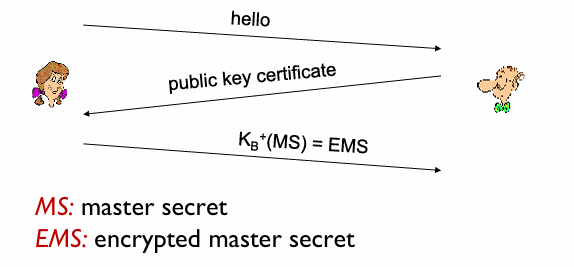
\includegraphics[width=0.5\linewidth]{immagini/handshake.png}
    \caption{Sequenza dei messaggi durante l'Handshake SSL.}
\end{figure}

\begin{urgentbox}{Difese integrate nell'Handshake}
\begin{itemize}
    \item \textbf{Perché scambiarsi due Nonce casuali?} Se non ci fossero i Nonce, Trudy potrebbe sniffare un'intera sessione (es. un ordine su Amazon) e inviare lo stesso esatto flusso di byte il giorno dopo (\textit{Connection Replay Attack}). Usando Nonce sempre diversi per ogni connessione, le chiavi generate saranno diverse ogni volta, rendendo i vecchi messaggi registrati da Trudy incomprensibili e non validi per il server.
    \item \textbf{Perché inviare il MAC di tutto l'handshake alla fine?} Per evitare un attacco \textit{Downgrade} (Man-in-the-Middle). Trudy potrebbe intercettare il primo messaggio \textit{ClientHello} e cancellare dalla lista gli algoritmi di crittografia forti, costringendo il server a sceglierne uno debole o bucato. Inviando il MAC di tutta la conversazione alla fine, Client e Server verificano che nessuno abbia alterato i messaggi iniziali inviati in chiaro.
\end{itemize}
\end{urgentbox}


\subsection*{Handshake SSL reale-- 6 passi}

\begin{center}
\renewcommand{\arraystretch}{1.4}
\begin{tabular}{|p{4.5cm}|c|p{4.5cm}|}
\hline
\textbf{Client} & & \textbf{Server} \\
\hline
& $\xrightarrow{\displaystyle\text{1. lista alg. + nonce client}}$ & \\
& $\xleftarrow{\displaystyle\text{2. alg. scelto + cert. + nonce server}}$ & \\
& $\xrightarrow{\displaystyle K_S^+(\mathit{pre\_master\_secret})}$ & \\
\multicolumn{3}{|c|}{\textit{4. entrambi derivano indipendentemente} $K_c, M_c, K_s, M_s$} \\
& $\xrightarrow{\displaystyle\text{5. MAC(handshake) cifrato}}$ & \\
& $\xleftarrow{\displaystyle\text{6. MAC(handshake) cifrato}}$ & \\
\multicolumn{3}{|c|}{\textcolor{okgreen}{\textbf{da qui tutto il traffico \`e cifrato e autenticato}}} \\
\hline
\end{tabular}
\end{center}

I passi 5--6 proteggono l'handshake da manomissioni (es. un attaccante che
avesse eliminato gli algoritmi forti nell'offerta del client sarebbe rilevato).

\newpage
\subsection{Fase 2: Key derivation (Derivazione delle Chiavi)}
In crittografia, è considerato molto pericoloso utilizzare la stessa chiave per operazioni diverse (es. usare la stessa chiave per cifrare e per calcolare il MAC) o per direzioni diverse.

\begin{defbox}{Il Key Block e le 4 Chiavi di Sessione}
A partire dal \texttt{pre\_master\_secret} e dai due Nonce, SSL utilizza una funzione pseudo-casuale (KDF) per generare un "Master Secret", dal quale si ritaglia un blocco di dati. Da questo blocco vengono derivate ben \textbf{4 chiavi distinte} e \textbf{2 Vettori di Inizializzazione (IV)}:
\begin{itemize}
    \item $K_c$: Chiave di cifratura per i dati inviati dal Client al Server.
    \item $M_c$: Chiave MAC per i dati inviati dal Client al Server.
    \item $K_s$: Chiave di cifratura per i dati inviati dal Server al Client.
    \item $M_s$: Chiave MAC per i dati inviati dal Server al Client.
\end{itemize}
Avere chiavi separate per direzione garantisce che un attaccante non possa prendere un pacchetto inviato dal client e "rifletterlo" al client stesso facendolo sembrare un pacchetto valido proveniente dal server.
\end{defbox}

\subsection{Fase 3 e 4: Data transfer(Record Protocol) e connection closure (garantisce chiusura connessione sicura)}
Non si può cifrare il flusso TCP come un unico blocco infinito, altrimenti il ricevitore non potrebbe controllare l'integrità dei dati (il MAC) fino alla fine della trasmissione. L'applicazione si bloccherebbe. SSL risolve il problema spezzando il flusso in \textbf{Record}.

\begin{notebox}{Formato dell'SSL Record}
Il flusso di dati viene frammentato in blocchi (max $\approx 16$ KB). Per ogni frammento:
\begin{enumerate}
    \item Si calcola il \textbf{MAC} sui dati in chiaro (usando $M_c$ o $M_s$).
    \item Si accoda il MAC al frammento.
    \item L'intero blocco (Dati + MAC) viene \textbf{cifrato} (usando $K_c$ o $K_s$).
    \item Viene aggiunta un'intestazione in chiaro (\textit{Record Header}) contenente: Tipo, Versione SSL e Lunghezza.
\end{enumerate}
\end{notebox}


\begin{urgentbox}{Difese del Record Protocol: Sequenze e Chiusure}
\begin{itemize}
    \item \textbf{Record Replay / Riordino:} Trudy potrebbe prendere un record valido e scambiarlo di posto o reinviarlo. Per evitarlo, nel calcolo del MAC viene inserito segretamente un \textbf{Numero di Sequenza}. Il numero di sequenza \textit{non viene trasmesso}, ma è tenuto a mente da mittente e ricevitore. Se Trudy sposta un record, il MAC calcolato dal ricevitore fallirà.
    \item \textbf{Truncation Attack:} Trudy potrebbe falsificare un segmento TCP con il flag \texttt{FIN} per forzare la chiusura prematura della connessione (es. prima che un bonifico sia completato). Per evitare questo, SSL usa il campo "Tipo" nell'Header. La vera chiusura avviene solo quando si riceve un Record speciale di "Chiusura Sicura" (Type 1), il cui MAC è verificabile crittograficamente.
\end{itemize}
\end{urgentbox}

\newpage
\newpage
\section{Sicurezza a livello di rete: IPsec e VPN}

A differenza di SSL che protegge una singola applicazione, \textbf{IPsec} opera al \textbf{livello 3 (Rete)}. 

Questo garantisce una \textit{copertura totale} (blanket coverage): qualsiasi payload trasportato dal livello di rete (segmenti TCP, UDP, messaggi ICMP) viene cifrato in modo del tutto trasparente per le applicazioni e gli utenti finali. 

Questa caratteristica lo rende la tecnologia fondante per le \textbf{VPN (Virtual Private Networks)}.

\subsection{Virtual Private Networks (VPN)}

Le organizzazioni e le aziende hanno spesso la necessità di creare reti private per garantire la massima sicurezza delle proprie comunicazioni interne. Poiché costruire un'infrastruttura fisica dedicata (con router e link separati) è proibitivo in termini di costi, si ricorre alle \textbf{VPN (Virtual Private Networks)}. 

Una VPN permette di instradare il traffico privato di un'istituzione attraverso l'Internet pubblico, cifrandolo prima che esca dalla rete sicura e mantenendolo logicamente separato da tutto il resto del traffico globale.
\begin{defbox}{Architetture VPN (Chi crea il tunnel/lavora?)}
Le VPN sono servizi basati sulla creazione di \textbf{tunnel cifrati} (tipicamente utilizzando IPsec in modalità Tunnel) tra due domini,  allo scopo di garantire comunicazioni sicure e riservate. Questa connessione protetta può essere stabilita e gestita in due architetture principali:
\begin{itemize}[leftmargin=*]
    \item \textbf{Site-to-Site (Tramite Router):} Usata per collegare tra loro intere reti locali (es. \textit{Headquarters} e \textit{Branch office}). In questo caso, \textbf{è il router che risolve la VPN per i client}. I computer all'interno della sede comunicano normalmente in chiaro; sarà il router di frontiera a farsi carico di incapsulare e cifrare i pacchetti prima di inviarli su Internet.
    \item \textbf{Remote Access (Tramite End-Host):} Usata dai lavoratori in mobilità (es. \textit{salesperson in hotel}). Essendo il computer connesso direttamente a una rete esterna (Internet), non c'è un router aziendale a fargli da scudo. Di conseguenza, il client \textbf{deve implementare dentro di sé la VPN}, eseguendo il software IPsec direttamente sul proprio laptop per creare un tunnel sicuro fino al router dell'azienda.
\end{itemize}
\end{defbox}

\newpage


\begin{figure}[H]
    \centering
    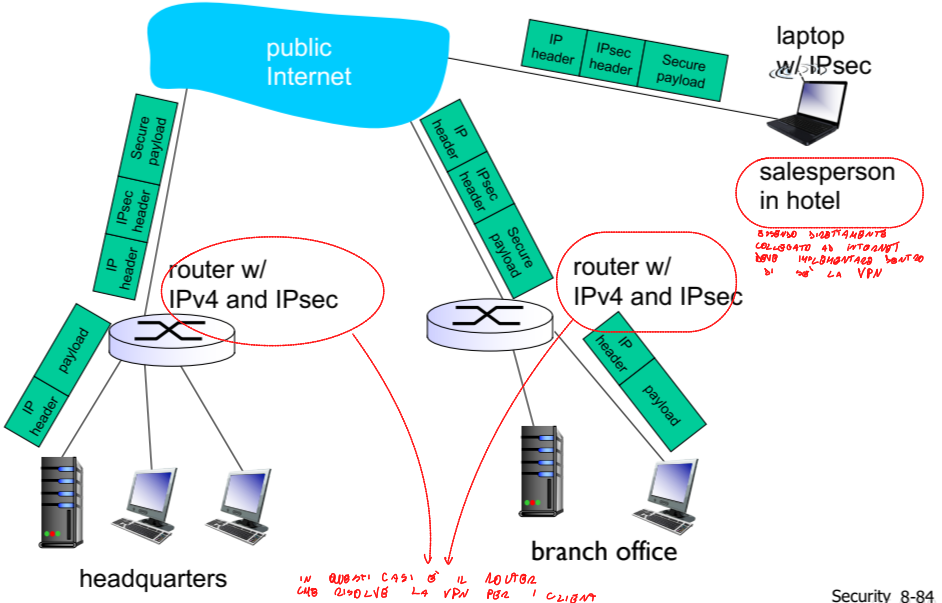
\includegraphics[width=0.8 \linewidth]{immagini/VPN.png}
    \caption{Topologia di una VPN: connessioni Site-to-Site tra router e Remote Access per host singoli.}
\end{figure}




\newpage
\subsection{Protocolli e Modalità di Funzionamento}
IPsec offre diversi servizi per mettere in sicurezza la comunicazione a livello di rete:
\begin{enumerate}
    \item Confidenzialità (riservatezza)
    \item Integrità dei dati
    \item Autenticazione dell'origine
    \item Prevenzione contro i \textit{replay attack}
\end{enumerate}

Questi servizi sono implementati tramite due protocolli principali:
\begin{center}
\begin{tabular}{llll}
\toprule
\textbf{Protocollo} & \textbf{Autent.} & \textbf{Riservatezza} & \textbf{Integrità} \\
\midrule
AH (Authentication Header) & \checkmark & $\times$ & \checkmark \\
ESP (Encapsulating Security Payload) & \checkmark & \checkmark & \checkmark \\
\bottomrule
\end{tabular}
\end{center}

L'implementazione pratica di questi protocolli dipende da \textit{chi} nella rete si fa carico di eseguire le operazioni crittografiche. Come illustrato nella topologia seguente, esistono due approcci principali:

\begin{itemize}
    \item \textbf{Implementazione sui Router (Edge routers IPsec-aware):} Corrisponde allo scenario a sinistra nell'immagine. L'onere della cifratura ricade interamente sui router di frontiera. I computer all'interno della rete locale (non \textit{IPsec-aware}) comunicano in chiaro come se si trovassero su una rete normale.
    
    Il router intercetta il traffico in uscita, applica IPsec in \textbf{Tunnel Mode}

    \item \textbf{Implementazione sugli Host (Hosts IPsec-aware):} Corrisponde allo scenario a destra nell'immagine. In questo caso, l'onere della cifratura ricade direttamente sui sistemi operativi degli end-system (i PC). I router intermedi si limitano al normale instradamento senza sapere nulla di IPsec. Questa implementazione lavora tipicamente in \textbf{Transport Mode}
\end{itemize}

\begin{notebox}{L'eccezione: Remote Access VPN}
Esiste uno scenario ibrido (visto nel concetto generale di VPN): il lavoratore in mobilità col proprio laptop. In questo caso, l'host del client funge esso stesso da "router di frontiera" virtuale: esegue IPsec in \textbf{Tunnel Mode} per collegarsi in modo sicuro all'Edge Router dell'azienda, nascondendo il proprio indirizzo IP locale.
\end{notebox}

% Placeholder Immagine: Edge routers vs Hosts
\begin{figure}[H]
    \centering
    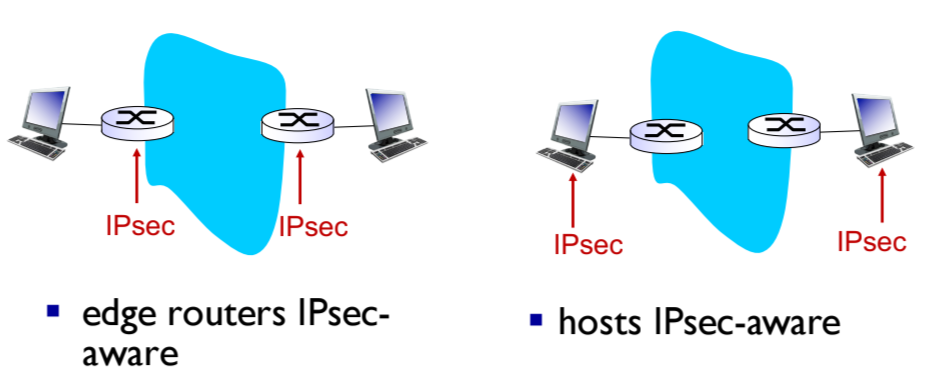
\includegraphics[width=0.6 \linewidth]{immagini/trans_mode.png}
    \caption{I due approcci implementativi di IPsec: a carico dei router di frontiera (sinistra, Tunnel Mode) o a carico degli host finali (destra, Transport Mode).}
\end{figure}


\begin{defbox}{Modalità IPsec: Transport Mode vs Tunnel Mode (Come si cifra?)}
IPsec offre due modalità  con cui manipola i datagrammi:

\begin{itemize}[leftmargin=*]
    \item \textbf{Transport Mode (Modalità Trasporto):} Viene cifrato e autenticato \textbf{solo il payload} (il segmento TCP/UDP) del pacchetto IP, mentre l'\textbf{header IP originale rimane in chiaro}. 
    \begin{itemize}
        \item \textit{Utilizzo:} Usato per comunicazioni dirette \textbf{Host-to-Host} (es. tra due server specifici che parlano tra loro in modo sicuro). Non è molto usato per le VPN classiche, poiché gli indirizzi IP sorgente e destinazione rimangono visibili a chi intercetta il traffico.
    \end{itemize}
    \item \textbf{Tunnel Mode (Modalità Tunnel):} Viene cifrato e autenticato l'\textbf{intero pacchetto IP originale} (sia l'header che il payload). Questo pacchetto completamente cifrato viene poi "imbustato" dentro un \textbf{nuovo pacchetto IP} con un nuovo header (che ha come mittente e destinatario gli indirizzi pubblici dei router/gateway VPN).
    \begin{itemize}
        \item \textit{Utilizzo:} È la modalità standard usata per le \textbf{VPN} (sia \textit{Site-to-Site} che \textit{Remote Access}). Nasconde completamente la topologia della rete interna aziendale, poiché gli indirizzi IP privati originali dei PC sono sigillati e invisibili all'interno del nuovo pacchetto.

        Questo offre un ulteriore livello di privacy: i router pubblici su Internet vedono solo lo scambio di pacchetti tra gli indirizzi IP esterni dei due gateway VPN. Come conseguenza pratica, \textit{"quello che arriva dal source arriva a destinazione senza sapere chi l'abbia mandato"}: gli indirizzi IP reali e le identità dei client all'interno della rete locale rimangono totalmente invisibili all'esterno.
    \end{itemize}
\end{itemize}
\end{defbox}

\begin{notebox}{Architetture VPN e Modalità IPsec}
Per non confondere questi quattro concetti dividiamoli in due categorie ben distinte: 

\vspace{0.2cm}
\textbf{1. Architetture VPN: CHI cifra e crea il tunnel?} \\
Determina quali apparati fisici si accollano il lavoro  di instaurare la connessione sicura e cifrare i dati.
\begin{itemize}[leftmargin=*]
    \item \textbf{Site-to-Site:} Il lavoro è fatto dai \textbf{Router di frontiera}. I PC all'interno della rete aziendale non sanno nulla della VPN e comunicano in chiaro. Sono i due router che catturano il traffico, lo cifrano, lo incapsulano e lo spediscono.
    \item \textbf{Remote Access:} Il lavoro è fatto dal \textbf{singolo Host remoto} (es. il PC del lavoratore con un software client VPN) e dal \textbf{Router aziendale}. Il PC del dipendente cifra i pacchetti in prima persona prima di immetterli su Internet.
\end{itemize}

\vspace{0.2cm}
\textbf{2. Modalità IPsec: COSA viene cifrato esattamente?} \\
Determina in che modo l'algoritmo matematico IPsec "imballa" il singolo pacchetto prima di spedirlo.
\begin{itemize}[leftmargin=*]
    \item \textbf{Tunnel Mode:} Viene cifrato l'\textbf{intero pacchetto IP originale} (sia l'Header con gli IP privati, sia i Dati). Questo "blocco" illeggibile viene poi inserito in un nuovo pacchetto IP con gli indirizzi pubblici dei router. È lo standard per le VPN perché nasconde le identità delle macchine interne.
    \item \textbf{Transport Mode:} Viene cifrato \textbf{solo il Payload} (i Dati di livello 4, es. TCP/UDP). L'Header IP originale rimane in chiaro. Chi intercetta il pacchetto su Internet non può leggerne il contenuto, ma può vedere esattamente quali due IP stanno comunicando. Usato solitamente per comunicazioni sicure dirette \textit{Host-to-Host}.
\end{itemize}
\end{notebox}


\newpage
\subsection{Associazioni di Sicurezza (SA) e Database}
Sebbene il protocollo IP di base sia di natura \textit{connectionless}, IPsec è rigorosamente \textbf{connection-oriented}. Questo perché il router (o l'host) mittente deve mantenere informazioni di stato per ogni comunicazione: deve sapere esattamente quali algoritmi e chiavi segrete utilizzare prima di poter instradare anche un solo pacchetto cifrato. Prima di inviare dati, i due nodi devono quindi stabilire preventivamente una connessione logica chiamata \textbf{Security Association (SA)}.

\begin{esempiobox}{Esempio Pratico: SA da R1 a R2}
Immaginiamo una topologia di rete con una sede centrale ("Headquarters", sottorete 172.16.1/24) collegata a Internet tramite il router di frontiera R1, che possiede l'indirizzo IP pubblico 200.168.1.100. Dall'altra parte del tunnel Internet, c'è una filiale ("Branch office", sottorete 172.16.2/24) protetta dal router R2, con indirizzo IP pubblico 193.68.2.23.

Affinché R1 possa inviare pacchetti cifrati a R2, deve essere stabilita una \textbf{Security Association (SA)} unidirezionale da R1 verso R2. Per questa specifica SA, il router R1 memorizzerà nel proprio database (SAD) i seguenti parametri essenziali:

\begin{itemize}
    \item \textbf{Identificatore SA (SPI):} Un indice numerico a 32 bit (Security Parameter Index) fondamentale per distinguere questa connessione dalle altre.
    \item \textbf{Interfaccia SA di origine:} L'indirizzo IP pubblico del router mittente R1 (200.168.1.100).
    \item \textbf{Interfaccia SA di destinazione:} L'indirizzo IP pubblico del router destinatario R2 (193.68.2.23).
    \item \textbf{Tipo di cifratura (Encryption):} L'algoritmo crittografico selezionato per garantire la confidenzialità (es. 3DES con CBC).
    \item \textbf{Chiave di cifratura:} La chiave simmetrica segreta da utilizzare in combinazione con l'algoritmo scelto.
    \item \textbf{Tipo di controllo di integrità:} L'algoritmo utilizzato per calcolare il MAC e garantire l'autenticazione (es. HMAC con MD5).
    \item \textbf{Chiave di autenticazione:} La chiave segreta utilizzata per firmare il MAC.
\end{itemize}
\end{esempiobox}

\begin{figure}[H]
    \centering
    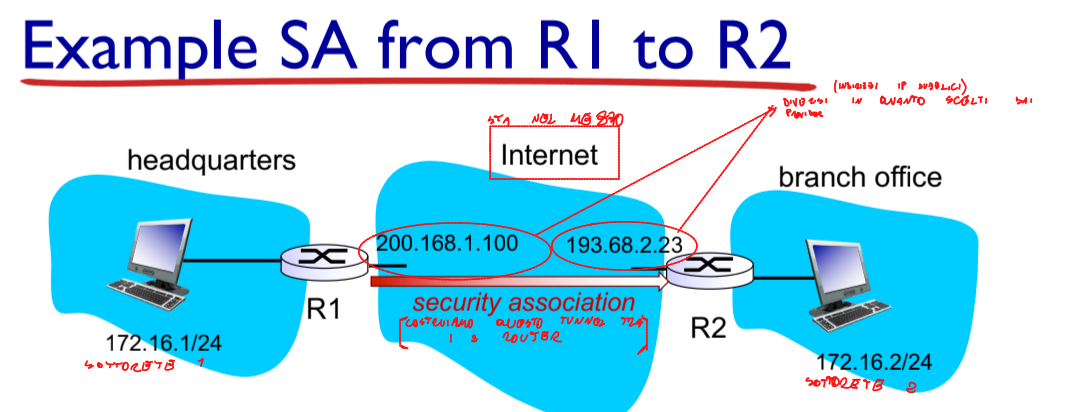
\includegraphics[width=0.9 \linewidth]{immagini/example.png}
    \caption{Rappresentazione di un'Associazione di Sicurezza (SA) unidirezionale tra due router di frontiera in una VPN.}
\end{figure}

\begin{defbox}{I Pilastri Logici: SA, SAD e SPD}
\begin{itemize}
    \item \textbf{SA (Security Association):} È una connessione \textit{simplex} (unidirezionale) tra l'entità mittente e quella destinataria. Essendo unidirezionale, per una normale comunicazione bidirezionale servono due SA separate. Una SA definisce l'interfaccia di origine e destinazione, gli algoritmi crittografici da usare, le chiavi condivise e un identificatore univoco a 32 bit chiamato \textbf{SPI (Security Parameter Index)}.
    
    \item \textbf{SAD (Security Association Database):} È il database in cui l'endpoint (es. il router) memorizza le informazioni di stato di tutte le SA attive. Quando un router riceve un pacchetto IPsec, legge il campo SPI dall'intestazione, lo usa come indice per cercare nel SAD e scopre esattamente \textbf{"come"} processare il datagramma (ovvero quali chiavi e algoritmi usare per decifrarlo).
    
    \item \textbf{SPD (Security Policy Database):} Contiene le regole di sicurezza (policy) della rete. Indica al router \textbf{"cosa"} fare con un datagramma (in arrivo o in uscita) in base all'IP sorgente/destinazione e alle porte. Il router consulta l'SPD per decidere se il pacchetto deve essere bloccato, fatto passare in chiaro, o se deve essere protetto con IPsec (in tal caso, l'SPD indicherà a sua volta quale SA presente nel SAD bisogna utilizzare).
\end{itemize}
\end{defbox}

\subsection{Struttura del Datagramma IPsec (Tunnel Mode con ESP)}
Per capire come i parametri della SA vengono applicati vediamo come è strutturato un pacchetto IPsec generato in modalità Tunnel con protocollo ESP.

% Placeholder Immagine: Struttura pacchetto IPsec (Slide 93)
\begin{figure}[H]
    \centering
    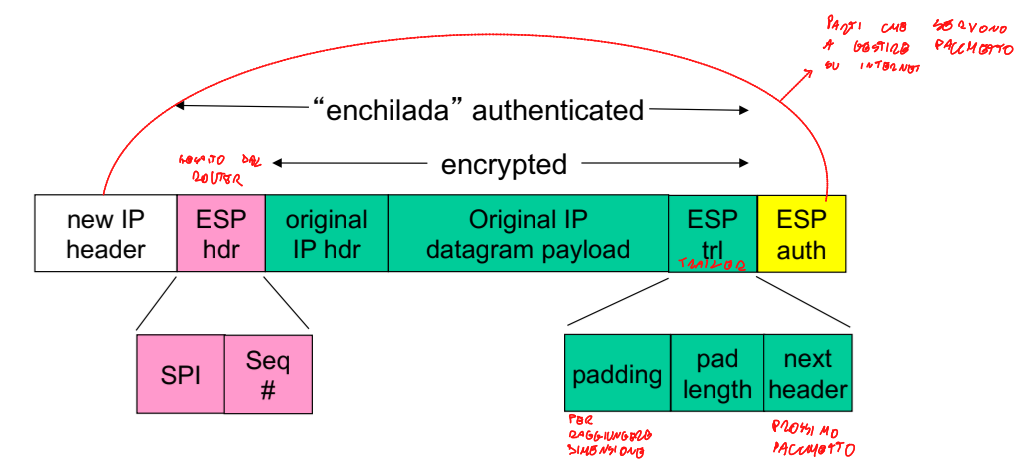
\includegraphics[width=0.8 \linewidth]{immagini/ipsec.png}
    \caption{Formato del datagramma IPsec in modalità Tunnel con protocollo ESP.}
\end{figure}

La costruzione di questo pacchetto (spesso definito gergalmente \textit{"enchilada"} per i suoi strati incapsulati) avviene nel seguente modo:
\begin{enumerate}
    \item \textbf{Dati originali:} Si parte dall'intero datagramma IP originale (Header IP interno + Payload applicativo).
    \item \textbf{ESP Trailer:} Viene aggiunto in coda. Contiene i \textbf{bit di padding} (necessari per allineare i dati per gli algoritmi di cifratura a blocchi come AES), la lunghezza del padding e il campo "Next Header".
    \item \textbf{Cifratura:} L'intero blocco fin qui ottenuto (Pacchetto IP Originale + ESP Trailer) viene \textbf{cifrato} utilizzando la chiave simmetrica specificata nella SA.
    \item \textbf{ESP Header:} Viene anteposto alla parte cifrata. È in chiaro e contiene:
    \begin{itemize}
        \item \textbf{SPI:} Fondamentale affinché il destinatario trovi la SA corretta nel SAD.
        \item \textbf{Sequence Number:} Un contatore che aumenta a ogni pacchetto, indispensabile per respingere i \textit{replay attack}.
    \end{itemize}
    \item \textbf{ESP Auth (MAC):} Per garantire l'integrità e l'autenticazione, viene calcolato un codice MAC (es. HMAC-MD5) su tutta la porzione composta da \textit{ESP Header + Parte Cifrata}. Questo codice viene accodato alla fine del pacchetto.
    \item \textbf{Nuovo IP Header:} Infine, per permettere al datagramma di essere instradato su Internet, viene inserito in testa un nuovo header IPv4 in chiaro, con gli indirizzi IP esterni dei due router VPN.
\end{enumerate}


\begin{urgentbox}{Prevenzione dei Replay Attack}
Oltre alla cifratura, IPsec si difende dagli attacchi di riproduzione (\textit{replay attack}) utilizzando i \textbf{Numeri di Sequenza} presenti nell'ESP header. 
All'avvio di una SA, il contatore parte da 0. Il mittente lo incrementa per ogni pacchetto inviato. Il destinatario memorizza una \textit{finestra} di numeri ricevuti validi. Se Trudy intercetta un pacchetto autentico e lo reinvia, il destinatario vedrà un numero di sequenza vecchio o già processato e scarterà il pacchetto immediatamente.
\end{urgentbox}

\subsection{Gestione delle Chiavi: Il protocollo IKE}
Per reti VPN molto grandi, inserire manualmente le chiavi per ogni singola SA nei router è materialmente impossibile. Per questo motivo IPsec utilizza il protocollo \textbf{IKE (Internet Key Exchange)}.


IKE automatizza la negoziazione su due fasi:
\begin{enumerate}[noitemsep]
  \item \textbf{Fase 1:} SA IKE bidirezionale (ISAKMP SA).
        Modalit\`a: \emph{aggressive} (meno msg) o \emph{main} (pi\`u sicura).
  \item \textbf{Fase 2:} coppia di SA IPsec negoziata tramite ISAKMP.
\end{enumerate}
Autenticazione IKE: \textbf{PSK} (pre-shared key) oppure \textbf{PKI} (certificati).

\newpage


\section{Sicurezza nelle Wireless LAN}

Le reti wireless (802.11) sono intrinsecamente meno sicure delle reti cablate perché il segnale viene trasmesso in broadcast (diffuso nell'aria): chiunque possieda un'antenna nel raggio di copertura può intercettare fisicamente i pacchetti.


% ─────────────────────────────────────────────────────────────────────────
\subsection{WEP -- Wired Equivalent Privacy}
% ─────────────────────────────────────────────────────────────────────────

Il WEP \`e stato il primo protocollo progettato per dare alle reti Wi-Fi un livello
di sicurezza ``equivalente'' a quello delle reti cablate. Nonostante le buone
intenzioni, si \`e rivelato \textbf{crittograficamente fallimentare}.

\subsubsection{Obiettivi di progetto}

\begin{defbox}{Obiettivi del WEP}
\begin{itemize}[noitemsep]
  \item \textbf{Crittografia simmetrica:} riservatezza, autorizzazione end-host, integrit\`a dei dati.
  \item \textbf{Auto-sincronizzante:} ogni pacchetto viene cifrato in modo \emph{indipendente},
        senza dover mantenere lo stato della sessione.
        Se un pacchetto va perso, il successivo si decifra comunque correttamente.
  \item \textbf{Efficienza:} implementabile sia in hardware che in software.
\end{itemize}
\end{defbox}

\subsubsection{I cifrari a flusso (stream cipher) -- base teorica}

Prima di spiegare il WEP \`e utile capire il meccanismo dei \textbf{stream cipher}.
A differenza dei cifrari a blocchi (come AES o DES), che cifrano blocchi fissi di dati,
uno stream cipher cifra il messaggio \emph{un byte alla volta}.

\begin{figure}[H]
    \centering
    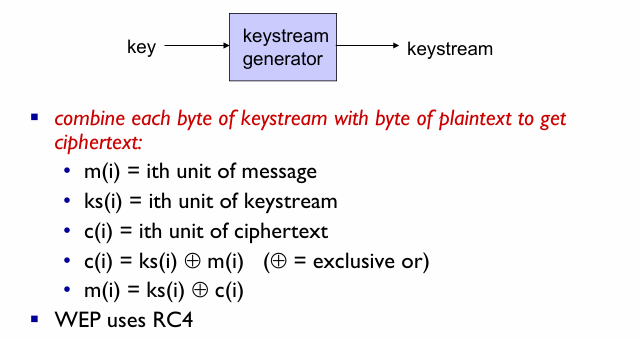
\includegraphics[width=0.7\linewidth]{immagini/slide_106.png}
    \caption{Funzionamento generale di un cifrario a flusso.}
    \label{fig:placeholder}
\end{figure}



\newpage
\begin{tcolorbox}[defbox, title=Meccanismo degli stream cipher]
\begin{enumerate}[noitemsep]
  \item Un \textbf{generatore di keystream} produce una sequenza pseudo-casuale di byte
        $ks_1, ks_2, ks_3, \ldots$ a partire da una chiave segreta.
  \item Ogni byte del messaggio $m_i$ viene combinato con il corrispondente byte del
        keystream $ks_i$ tramite \textbf{XOR} (OR esclusivo):
        \[
          c_i = ks_i \oplus m_i \qquad \text{(cifratura)}
        \]
  \item La decifratura \`e identica (XOR \`e l'inverso di se stesso):
        \[
          m_i = ks_i \oplus c_i \qquad \text{(decifratura)}
        \]
\end{enumerate}
Il WEP usa l'algoritmo \textbf{RC4} come generatore di keystream.
\end{tcolorbox}

\paragraph{Perch\'e ogni pacchetto deve essere cifrato separatamente?}


Se si usasse un keystream continuo (continuando da dove si era rimasti nel pacchetto
precedente), ogni pacchetto \emph{non} sarebbe cifrato in modo indipendente:
basterebbe sapere dove si era fermi per il pacchetto $n$ per decifrare il pacchetto $n{+}1$.
Soluzione del WEP: per ogni pacchetto si \textbf{reinizializza il generatore RC4}
con la chiave segreta pi\`u un nuovo \textbf{IV (Initialization Vector)}.

\newpage
\subsubsection{Cifratura WEP -- dettaglio}

WEP usa il cifrario a flusso \textbf{RC4}:

\begin{center}
\begin{tikzpicture}[
  box/.style={draw=uniboblue,fill=unibolight,rounded corners=3pt,
    minimum width=2.5cm,minimum height=0.65cm,font=\small,align=center},
  arr/.style={-Latex,thick,draw=uniboblue!80}]
  \node[box](ks){$K_S$ (104 bit)};
  \node[box,right=0.5cm of ks](iv){IV (24 bit)};
  \node[box,right=1.5cm of iv](gen){Generatore\\keystream RC4};
  \node[box,right=1.5cm of gen](ksout){$k_1 k_2 \ldots$};
  \node[box,below=0.9cm of ksout](data){Dati + ICV};
  \node[box,right=1.5cm of data](xor){XOR\;$c_i = k_i \oplus d_i$};
  \draw[arr](ks)--(gen);\draw[arr](iv)--(gen);
  \draw[arr](gen)--(ksout);\draw[arr](ksout)--(xor);
  \draw[arr](data)--(xor);
\end{tikzpicture}
\end{center}

\begin{tcolorbox}[defbox, title=Processo di cifratura WEP (passo per passo)]
\begin{enumerate}[noitemsep]
  \item \textbf{ICV (Integrity Check Value):} il mittente calcola un hash/CRC
        a 4 byte sui dati del frame $\to$ garantisce l'integrit\`a.
  \item \textbf{Chiave da 128 bit:} la chiave segreta condivisa \`e a \textbf{104 bit};
        il mittente genera un \textbf{IV da 24 bit} (diverso per ogni pacchetto)
        e lo concatena, ottenendo 128 bit totali.
  \item \textbf{Generazione keystream:} la chiave da 128 bit entra nel generatore
        pseudo-casuale RC4 $\to$ produce il keystream.
  \item \textbf{XOR:} i byte del keystream vengono XOR-ati con \emph{(dati + ICV)}
        $\to$ si ottiene il ciphertext.
  \item \textbf{Trasmissione:} il pacchetto inviato contiene:
        IV in chiaro (nel header 802.11, affinchè il destinatario sappia come ricreare keystream corretto) + KeyID + dati cifrati.
\end{enumerate}
\end{tcolorbox}

\begin{figure}[H]
    \centering
    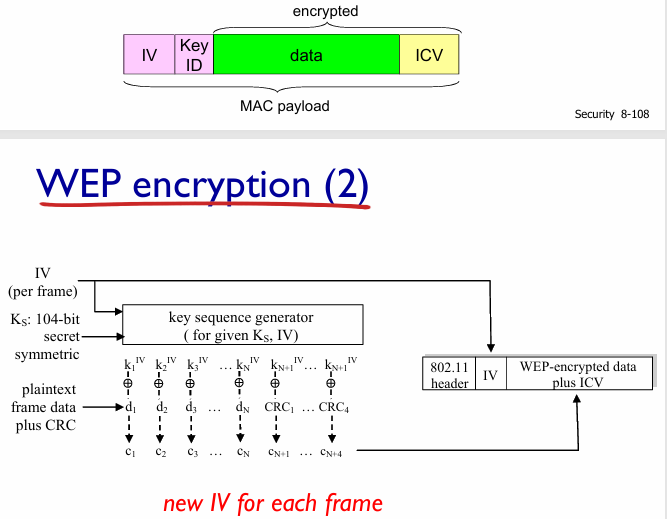
\includegraphics[width=0.7\linewidth]{immagini/slide_108.png}
    \caption{schema completo protocollo WEP 802.11: generazione keystream per ciascun frame con IV specifico}
    \label{fig:placeholder}
\end{figure}

La figura mostra il funzionamento frame per frame: per ogni frame $n$ si usa
$(K_S \| IV_n)$ come seme per RC4; il keystream prodotto viene XOR-ato con
$(d_1 d_2 \ldots d_N \| CRC_1 \ldots CRC_4)$.
L'IV \`e trasmesso \textbf{in chiaro} nell'header del frame 802.11.

\subsection*{Decifratura WEP}

\begin{enumerate}[noitemsep]
  \item Il ricevitore \textbf{estrae l'IV} dall'header del pacchetto (in chiaro).
  \item Immette IV + chiave segreta condivisa nel generatore RC4 $\to$ ottiene
        lo \emph{stesso identico keystream} del mittente.
  \item XOR del keystream con il ciphertext $\to$ recupera dati + ICV.
  \item \textbf{Verifica ICV:} Lo ricalcola sui dati ottenuti e lo confronta
        con l'ICV ricevuto $\to$ se non coincidono, il pacchetto \`e corrotto o manomesso.
\end{enumerate}
\textbf{Nota:} l'integrit\`a qui si basa su CRC/ICV, non su un MAC crittografico
robusto (HMAC), il che \`e un'ulteriore debolezza.


\subsection*{Autenticazione WEP}

L'autenticazione WEP usa un meccanismo \textbf{challenge-response} basato su nonce:
\begin{enumerate}[noitemsep]
  \item Il client invia una \textit{authentication request}.
  \item L'AP risponde con un nonce (128 byte di sfida).
  \item Il client cifra il nonce con la chiave condivisa e lo rispedisce.
  \item L'AP verifica: se il nonce decifrato corrisponde, l'autenticazione \`e riuscita.
\end{enumerate}
\textbf{Limitazione:} non tutti gli AP richiedono autenticazione anche con WEP attivo.

\subsection{La vulnerabilit\`a critica: attacco al keystream WEP}


\begin{urgentbox}{Perch\'e il WEP \`e fallimentare -- L'attacco al keystream}
La debolezza fatale \`e la \textbf{brevit\`a dell'IV} (soli 24 bit):

\begin{enumerate}[noitemsep]
  \item Esistono $2^{24} \approx 16$ milioni di IV possibili.
  \item In una rete trafficata, gli IV si \textbf{esauriscono} e si \textbf{ripetono}
        anche dopo poche decine di minuti.
  \item L'IV \`e trasmesso \textbf{in chiaro}: Trudy (l'attaccante) rileva
        il riutilizzo immediatamente.
\end{enumerate}

\textbf{L'attacco:}
\begin{enumerate}[noitemsep]
  \item Trudy induce Alice a cifrare un testo noto $d_1 d_2 d_3 \ldots$
        (es. iniettando traffico noto o sfruttando pacchetti ARP il cui contenuto \`e prevedibile).
  \item Trudy osserva il ciphertext: $c_i = k_i^{IV} \oplus d_i$.
  \item Poich\'e conosce sia $c_i$ che $d_i$, \textbf{ricava il keystream}: $k_i^{IV} = c_i \oplus d_i$.
  \item La prossima volta che l'IV viene riutilizzato, Trudy conosce gi\`a il keystream
        corrispondente $\Rightarrow$ \textbf{decifra istantaneamente tutti i pacchetti
        inviati con quell'IV}.
\end{enumerate}
In pratica, con strumenti liberamente disponibili (es. \texttt{aircrack-ng}),
una chiave WEP a 104 bit si rompe in \textbf{pochi minuti}.
\end{urgentbox}

\newpage
% ─────────────────────────────────────────────────────────────────────────
\subsection{802.11i (WPA2) -- La soluzione definitiva}
% ────────────────────────────────────────────────────────────────────────

\begin{tcolorbox}[keybox, title=802.11i -- Miglioramenti fondamentali rispetto al WEP]
\begin{description}[leftmargin=3.5cm, style=nextline, noitemsep]
  \item[\textcolor{okgreen}{Cifratura robusta}]
    Abbandona RC4 in favore di \textbf{AES} (in modalit\`a CCMP), un cifrario a blocchi
    moderno e crittograficamente solido.
  \item[\textcolor{okgreen}{Chiavi dinamiche}]
    Nessuna chiave statica. Per ogni sessione di ogni client si derivano
    \textbf{Temporal Keys (TK)} tramite un 4-way handshake che le rinnova
    frequentemente, rendendo impossibile collezionare dati a sufficienza per
    rompere la cifratura.
  \item[\textcolor{okgreen}{AS separato}]
    L'autenticazione reale \`e delegata a un \textbf{Authentication Server (AS)}
    separato dall'AP (Access point). L'AP funge solo da ``pass-through'' per i messaggi EAP.
    Questo permette una gestione centralizzata e robusta delle identit\`a.
\end{description}
\end{tcolorbox}

\subsubsection{Le quattro fasi di 802.11i}

\begin{figure}[H]
    \centering
    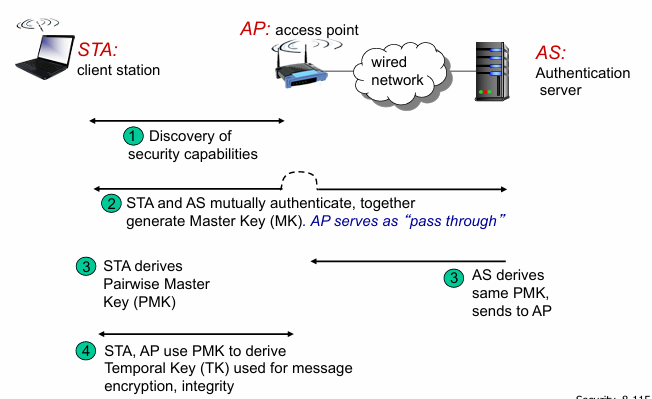
\includegraphics[width=0.7\linewidth]{immagini/Immagine 2026-03-14 112153.png}
    \caption{
La foto mostra i tre attori: \textbf{STA} (client), \textbf{AP} (access point),
\textbf{AS} (authentication server, connesso alla rete cablata).}
    \label{fig:placeholder}
\end{figure}


\begin{tcolorbox}[defbox, title=Le 4 fasi di 802.11i]
\begin{description}[leftmargin=1cm, style=nextline]
  \item[\textbf{Fase 1 -- Discovery delle capacit\`a di sicurezza}]
    STA e AP si scambiano i protocolli di sicurezza supportati
    (cifratura, autenticazione). Negoziano quale usare.

  \item[\textbf{Fase 2 -- Autenticazione mutua STA $\leftrightarrow$ AS}]
    STA e AS si autenticano a vicenda tramite EAP. L'AP fa da
    ``passacarte'' (pass-through) per i messaggi EAP.
    Al termine, STA e AS hanno derivato una \textbf{Master Key (MK)}.

  \item[\textbf{Fase 3 -- Derivazione della Pairwise Master Key (PMK)}]
    Sia STA che AS derivano in modo indipendente la \textbf{PMK} dalla MK.
    L'AS invia la PMK all'AP in modo sicuro.

  \item[\textbf{Fase 4 -- Derivazione della Temporal Key (TK) via 4-Way Handshake}]
    STA e AP usano la PMK per derivare la \textbf{TK} (usata per cifratura e
    integrit\`a del traffico dati). Il 4-way handshake garantisce che
    entrambe le parti abbiano davvero la PMK e che le TK siano fresche.
\end{description}
\end{tcolorbox}

\subsubsection{EAP -- Extensible Authentication Protocol}


EAP \`e un protocollo di autenticazione \textbf{end-to-end} tra client mobile e AS,
trasportato su due link distinti:

\begin{center}
\begin{tabular}{llll}
\toprule
\textbf{Tratto} & \textbf{Protocollo} & \textbf{Livello} & \textbf{Stack} \\
\midrule
STA $\leftrightarrow$ AP & EAP over LAN (\textbf{EAPoL}) & Link & IEEE 802.11 \\
AP $\leftrightarrow$ AS  & \textbf{RADIUS} & Trasporto/rete & UDP/IP \\
\bottomrule
\end{tabular}
\end{center}


\begin{esempiobox}{Confronto WEP vs.\@ 802.11i}
\begin{center}
\begin{tabular}{lll}
\toprule
\textbf{Caratteristica} & \textbf{WEP} & \textbf{802.11i (WPA2)} \\
\midrule
Cifratura & RC4 (stream) & AES-CCMP (blocchi) \\
Chiavi & Statiche, 104 bit & Dinamiche (TK per sessione) \\
IV & 24 bit, in chiaro & Nonce a 48 bit, sequenziato \\
Integrit\`a & CRC/ICV (debole) & CCMP con CBC-MAC (forte) \\
Autenticazione & Challenge-response debole & EAP mutua con AS separato \\
Sicurezza & \textcolor{alertred}{\textbf{Rotta (minuti)}} & \textcolor{okgreen}{\textbf{Robusta}} \\
\bottomrule
\end{tabular}
\end{center}
\end{esempiobox}










\newpage

% ══════════════════════════════════════════════════════════════════════════
\section{Sicurezza operativa: Firewall e IDS}
% ══════════════════════════════════════════════════════════════════════════

Anche applicando protocolli crittografici robusti come IPsec o SSL,
una rete \`e esposta a pericoli provenienti da Internet.
Il \textbf{firewall} e l'\textbf{IDS} costituiscono la prima linea di difesa
a livello operativo.

% ─────────────────────────────────────────────────────────────────────────
\subsection{Firewall -- Concetto }
% ─────────────────────────────────────────────────────────────────────────
\begin{figure}[H]
    \centering
    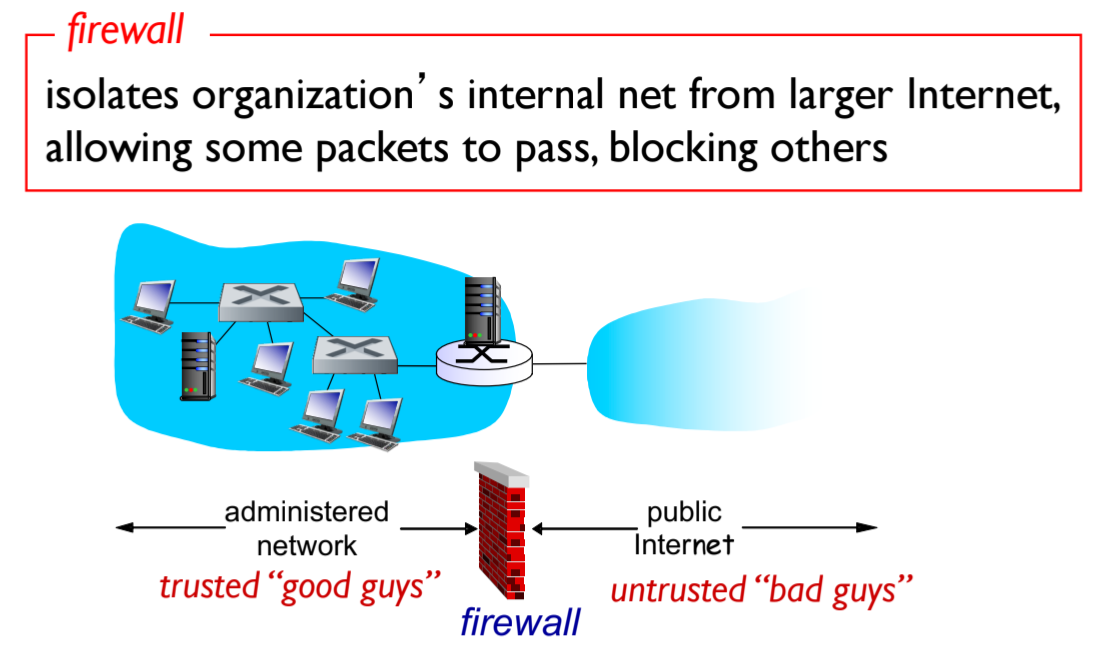
\includegraphics[width=0.5\linewidth]{immagini/firewall.png}
    \caption{
Concetto di base: il firewall isola la rete interna (trusted) da Internet (untrusted), filtrando i pacchetti in entrata e in uscita.}
    \label{fig:placeholder}
\end{figure}


\begin{defbox}{Firewall}
Un \textbf{firewall} \`e un sistema (hardware o software) che \textbf{isola} la rete
interna di un'organizzazione da Internet, lasciando passare alcuni pacchetti e
bloccandone altri in base a regole configurate dall'amministratore.
\end{defbox}


\begin{esempiobox}{Architettura DMZ per la protezione dei servizi esposti}
\textbf{La Minaccia (Privilege Escalation):} \\
I server che offrono servizi al pubblico (es. Web, DNS, Email) sono costantemente esposti ad attacchi da Internet. Se questi server venissero collocati direttamente all'interno della rete locale (\textit{Trusted}), un malintenzionato che riuscisse a comprometterne uno potrebbe sfruttarlo come "testa di ponte" per ottenere i privilegi di amministratore e avere libero accesso a tutta la rete interna aziendale.

\textbf{Soluzione 1: Firewall a tre interfacce (Three-homed Firewall\footnote{Vedi un esempio nella section \ref{IDS}})} \\
Per isolare questo rischio, si crea una \textbf{DMZ (Demilitarized Zone)}, ovvero una sottorete perimetrale isolata. Si utilizza un firewall dotato fisicamente di tre interfacce di rete:
\begin{itemize}
    \item \textbf{Rete Esterna (Untrusted):} Collegata a Internet.
    \item \textbf{DMZ:} La zona "cuscinetto" dove risiedono i server esposti al pubblico.
    \item \textbf{Rete Interna (Trusted):} La LAN aziendale, strettamente protetta.
\end{itemize}
\textit{Regola d'oro:} Il firewall permette il traffico da Internet verso la DMZ, ma \textbf{blocca} rigorosamente qualsiasi connessione iniziata dalla DMZ verso la Rete Interna.

\newpage
\textbf{Soluzione 2: Implementazione tramite Switch (VLAN) o Doppio Firewall} \\
Se non si dispone di un firewall con tre porte fisiche dedicate, l'isolamento della DMZ può essere implementato come segue:
\begin{itemize}
    \item \textbf{Logicamente (tramite Switch e VLAN):} Utilizzando uno switch \textit{Layer 3} configurato con VLAN separate. Lo switch isola il dominio di broadcast della DMZ da quello della rete interna, instradando il traffico in modo sicuro.
\end{itemize}
\end{esempiobox}


\subsection{Perchè servono i firewall}
\begin{urgentbox}
    
\begin{itemize}[noitemsep]
  \item \textbf{Prevenzione DoS -- SYN flooding:}
        un attaccante apre migliaia di connessioni TCP bogus (SYN senza completare
        il 3-way handshake), saturando la tabella delle connessioni del server
        e impedendo connessioni legittime.
  \item \textbf{Blocco modifiche illegali ai dati interni:}
        es. impedire a Trudy di sostituire la homepage del server web interno.
  \item \textbf{Accesso autorizzato all'interno:}
        solo utenti/host autenticati possono accedere a risorse sensibili.
\end{itemize}
Esistono tre tipologie principali: \textbf{stateless packet filter},
\textbf{stateful packet filter}, \textbf{application gateway}((applica regole di livello applicazione).
\end{urgentbox}

% ─────────────────────────────────────────────────────────────────────────
\subsection{1. Packet Filter Stateless}
% ─────────────────────────────────────────────────────────────────────────


\begin{defbox}{Stateless Packet Filtering}
\begin{itemize}[noitemsep]
  \item La rete interna \`e connessa a Internet tramite un \textbf{router-firewall}.
  \item Il router analizza ogni pacchetto \textbf{in modo indipendente}(anche all'interno di una stessa sessione) e decide
        se fare forward o drop(cestina).
  \item La decisione si basa solo sugli header:
\end{itemize}
\begin{center}
\small
\setlength{\tabcolsep}{3pt}
\begin{tabular}{ll}
\toprule
\textbf{Campo analizzato} & \textbf{Esempio di regola} \\
\midrule
IP sorgente & Blocca traffico da IP non autorizzati \\
IP destinazione & Permetti solo verso il web server \\
Porta TCP/UDP src e dst & Blocca porta 23 (Telnet) \\
Tipo ICMP & Blocca messaggi di stato rete:ping broadcast (anti-Smurf DoS) \\
Flag TCP (SYN, ACK) & Blocca SYN in ingresso (no new connections) \\
\bottomrule
\end{tabular}
\end{center}
\end{defbox}

\newpage
\subsubsection{Esempi di regole stateless}

\begin{esempiobox}{Esempi concreti di regole stateless}
    
\textbf{Esempio 1:blocco UDP+Telnet (bloccon traffico entrante ed uscente )}

Blocca IP protocollo = 17 (UDP) E porta src/dst = 23.\\
$\Rightarrow$ Blocca tutti i flussi UDP in ingresso/uscita \textbf{e} tutte le connessioni Telnet.


\medskip
\textbf{Esempio 2:Blocca TCP in ingresso con ACK\,=\,0.\\ (impediamo dall'esterno la chiusura di una sessione)}

$\Rightarrow$ Impedisce ai client esterni di avviare connessioni TCP verso l'interno
(il primo pacchetto SYN ha ACK\,=\,0), ma \textbf{permette} ai client interni
di connettersi all'esterno (i pacchetti di risposta hanno ACK\,=\,1).
\end{esempiobox}


\subsubsection{Access Control List (ACL)}


La \textbf{ACL} \`e la tabella di regole del firewall stateless, applicata
\textbf{dall'alto verso il basso}: la prima regola che combacia con il pacchetto
determina l'azione (allow/deny). L'ultima regola \`e sempre un
\emph{deny all} implicito.

Le regole in alto vengono applicate per prime. Se ci sono quindi due regole conflittuali viene applicata prima quella più in alto.

\begin{center}
\small
\renewcommand{\arraystretch}{1.3}
\begin{tabular}{ccccccc}
\toprule
\textbf{Azione} & \textbf{Proto} & \textbf{IP src} & \textbf{IP dst} &
\textbf{P. src} & \textbf{P. dst} & \textbf{Flag} \\
\midrule
allow & TCP & 222.22/16 & esterno & $>$1023 & 80 & any \\
allow & TCP & esterno & 222.22/16 & 80 & $>$1023 & ACK \\
allow & UDP & 222.22/16 & esterno & $>$1023 & 53 & -- \\
allow & UDP & esterno & 222.22/16 & 53 & $>$1023 & -- \\
\rowcolor{red!15}\textbf{deny} & \textbf{all} & \textbf{all} &
\textbf{all} & \textbf{all} & \textbf{all} & \textbf{all} \\
\bottomrule
\end{tabular}
\end{center}

\vspace{0.3em}
\textbf{Lettura:} le prime due righe permettono navigazione web (HTTP) La prima infatti permette invio di dati verso esterno a chiunque. 
La seconda permette la ricezione; 

le successive due permettono query DNS (invio e ricezione);

l'ultima riga blocca tutto il resto che passa attraverso il firewall(sia dall'interno verso esterno che il contrario).

\begin{esempiobox}{policy comuni con ACL}
\begin{itemize}[noitemsep]
  \item \textbf{Nessun accesso web dall'interno (verso l'esterno):}
        dico al firewall  di effettuare un drop pacchetti uscenti verso qualsiasi IP, porta 80.
  \item \textbf{Solo web server pubblico raggiungibile dall'esterno:}
        drop TCP SYN in ingresso verso qualsiasi IP tranne 130.207.244.203:80 (web server pubblico dell'istituzione). A questa quindi è concesso l'accesso dall'esterno.
  \item \textbf{Blocca web-radio} (consumano banda):
        drop UDP in ingresso (eccetto DNS e router broadcast).
  \item \textbf{Prevenire Smurf DoS attack (attacca indirizzo brodcast di aziende):}
        drop pacchetti ICMP verso indirizzi broadcast (es. 130.207.255.255).
  \item \textbf{Blocca traceroute:}
        drop ICMP TTL-expired in uscita.
\end{itemize}
\end{esempiobox}

% ─────────────────────────────────────────────────────────────────────────
\subsection{2. Packet Filter Stateful}
% ─────────────────────────────────────────────────────────────────────────

Il filtro stateless \`e grezzo: ammette pacchetti ACK senza SYN precedente (ovvero senza aver aperto connessione tra i due che stanno interagendo).\\
Il filtro \textbf{stateful} traccia lo stato di ogni connessione TCP (ovvero di ciascuno degli stati intermedi nella connessione attivando regole determinate ad ogni sessione):
\begin{itemize}[noitemsep]
  \item Monitora setup (SYN) e teardown (FIN).
  \item Verifica che ogni pacchetto in ingresso corrisponda a una connessione attiva.
  \item Scade automaticamente le connessioni inattive.
  \item La ACL viene estesa con una colonna ``check connection table'' (flag $\times$).
\end{itemize}

\begin{center}
\small
\renewcommand{\arraystretch}{1.3}
\begin{tabular}{cccccccc}
\toprule
\textbf{Azione} & \textbf{Proto} & \textbf{IP src} & \textbf{IP dst} & \textbf{P. src} & \textbf{P. dst} & \textbf{Flag} & \textbf{Check Conn.} \\
\midrule
allow & TCP & 222.22/16 & esterno & $>$1023 & 80 & Any & -- \\
allow & TCP & esterno & 222.22/16 & 80 & $>$1023 & ACK & x \\
allow & UDP & 222.22/16 & esterno & $>$1023 & 53 & -- & -- \\
allow & UDP & esterno & 222.22/16 & 53 & $>$1023 & -- & x \\
\rowcolor{red!15}\textbf{deny} & \textbf{all} & \textbf{all} & \textbf{all} & \textbf{all} & \textbf{all} & \textbf{all} & \textbf{all} \\
\bottomrule
\end{tabular}
\end{center}
\begin{notebox}{Significato della "X" (Check Conn.) nei Firewall Stateful}
    Nei packet filter stateful, la colonna "Check Connection" serve a indicare se il firewall deve consultare la sua tabella interna degli stati TCP.
        \begin{itemize}
            \item \textbf{Se c'è la "X":} Il firewall fa passare il pacchetto \textbf{solo se} verifica che faccia parte di una connessione già aperta e attiva  (ad esempio, la risposta legittima di un sito web a una richiesta precedente).
            \item \textbf{Se NON c'è la "X":} La regola si applica direttamente senza controllare la memoria. Questo si usa tipicamente per autorizzare l'apertura di \textit{nuove} connessioni (es. il primo pacchetto SYN inviato verso l'esterno).
        \end{itemize}
\end{notebox}

\newpage
% ─────────────────────────────────────────────────────────────────────────
\subsection{3. Application Gateway (Proxy)}
% ─────────────────────────────────────────────────────────────────────────


I packet filter (stateless o stateful) si fermano al livello di trasporto (L4).
Se si vuole filtrare in base ai \textbf{dati dell'applicazione}
(es. permettere Telnet/SSH solo ad alcuni utenti autenticati),
occorre un \textbf{Application Gateway} (detto anche \textit{proxy}).

\begin{tcolorbox}[defbox, title=Funzionamento dell'Application Gateway]
\begin{enumerate}[noitemsep]
  \item Il router/firewall blocca \emph{tutte} le connessioni dirette verso l'esterno.
  \item L'utente interno deve connettersi \textbf{prima al Gateway} (es. via Telnet).
  \item Il Gateway \textbf{autentica} l'utente a livello applicativo
        (es. verifica username/password Telnet).
  \item Se autorizzato, il Gateway instanzia una \textbf{seconda connessione separata}
        verso il server esterno e fa da ``ponte'': ri-trasmette i dati tra le due connessioni.
  \item Il router(firewall) blocca qualsiasi connessione che non origini dal Gateway, quindi si trova in mezzo alla connessione 2 effettuata dal gateway verso l'esterno.
\end{enumerate}
\end{tcolorbox}

Non è più il client che passa dal firewall, ma c'è un intermediario (il Gateway) che fa da intermediario. 

\begin{figure}[H]
    \centering
    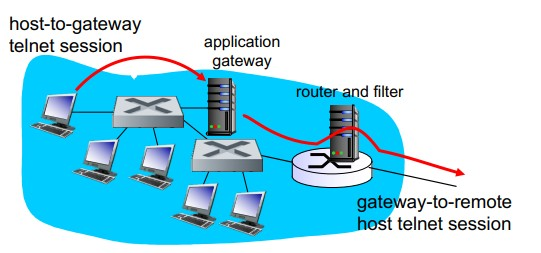
\includegraphics[width=0.5\linewidth]{immagini/secure.jpg}
    \caption{}
    \label{fig:placeholder}
\end{figure}

\newpage
\subsection{Confronto delle tre tipologie di firewall}
\begin{table}[hbt!]
\centering
\renewcommand{\arraystretch}{1.5} % Aumenta leggermente lo spazio tra le righe per leggibilità
\begin{tabular}{|p{3cm}|p{2cm}|p{3.5cm}|c|p{4cm}|}
\hline
\textbf{Tipo di Firewall} & \textbf{Livello OSI} & \textbf{Cosa Ispeziona?} & \textbf{Memoria} & \textbf{Pro / Contro principali} \\ \hline
\textbf{Stateless Packet Filter} & 3 (Rete) e 4 (Trasporto) & Solo le intestazioni in modo isolato (IP, porte, flag TCP). & \textbf{NO} & \textbf{Pro:} Molto veloce e leggero.\newline \textbf{Contro:} Grezzo, non riconosce i pacchetti fuori contesto. \\ \hline
\textbf{Stateful Packet Filter} & 3 (Rete) e 4 (Trasporto) & Intestazioni + tracciamento delle connessioni (SYN, ACK, FIN). & \textbf{SÌ} & \textbf{Pro:} Più intelligente, blocca risposte non richieste.\newline \textbf{Contro:} Richiede più risorse per mantenere la tabella degli stati. \\ \hline
\textbf{Application Gateway (Proxy)} & 7 (Applicazione) & Dati e payload a livello applicativo (crea un ponte/intermediario). & \textbf{N/A} & \textbf{Pro:} Massima sicurezza, permette autenticazione profonda.\newline \textbf{Contro:} Lento, pesante e serve un proxy per ogni singola app. \\ \hline
\end{tabular}
\caption{Confronto delle tre tipologie principali di Firewall}
\label{tab:confronto_firewall}
\end{table}
% ─────────────────────────────────────────────────────────────────────────
\subsection{Limitazioni dei Firewall}
% ─────────────────────────────────────────────────────────────────────────


\begin{urgentbox}{Limitazioni fisiche dei Firewall}
\begin{itemize}[noitemsep]
  \item \textbf{IP Spoofing:} il router non pu\`o sapere se il pacchetto
        ``proviene davvero'' dall'IP sorgente dichiarato o se \`e falsificato. La risposta ai pacchetti mandati dai malintenzionati arriva all'IP di colui di cui è stato fatto spoofing.
  \item \textbf{UDP -- politica tutto-o-niente:} i filtri UDP sono difficili:
        o si blocca tutto UDP (e si perdono servizi come DNS, NTP\ldots)
        o si lascia passare tutto.
  \item \textbf{Scalabilit\`a degli Application Gateway:}
        se 10 applicazioni richiedono un proxy dedicato, occorrono 10 gateway;
        i client devono essere configurati esplicitamente per ciascuno.
  \item \textbf{Trade-off ineliminabile:} pi\`u si aumenta il filtraggio,
        pi\`u si riduce l'apertura verso il mondo esterno e viceversa.
  \item \textbf{Limiti pratici:} molti siti molto protetti subiscono comunque attacchi
        (attacchi dall'interno, ingegneria sociale).
\end{itemize}
\end{urgentbox}

\newpage
% ─────────────────────────────────────────────────────────────────────────
\subsection{IDS -- Intrusion Detection Systems}
\label{IDS}
% ─────────────────────────────────────────────────────────────────────────
{IDS vs Packet Filtering: il packet filter opera solo sugli header, l'IDS esegue deep packet inspection e analisi di correlazione tra pi\`u sessioni.

Il firewall \`e la ``porta blindata'' che controlla le intestazioni, ma non
guarda cosa c'\`e \emph{dentro} il pacchetto.
Se un pacchetto \`e formalmente corretto (es. destinato alla porta 80 del web server),
il firewall lo fa passare \textbf{anche se il payload contiene codice malevolo}.

\begin{defbox}{IDS -- Deep Packet Inspection}
\begin{description}[leftmargin=3.5cm, style=nextline, noitemsep]
  \item[\textcolor{uniboblue}{Packet filter}]
    Opera \emph{solo} sugli header TCP/IP; nessuna correlazione tra sessioni distinte.
  \item[\textcolor{uniboblue}{IDS}]
    Esegue \textbf{Deep Packet Inspection (DPI)}: analizza il contenuto reale
    (payload applicativo) e il contesto:
    \begin{itemize}[noitemsep]
      \item \textbf{Firme (signatures):} confronta stringhe di byte con un database
            di virus, malware, exploit noti (es. pattern di buffer overflow).
      \item \textbf{Correlazione (euristiche):} analizza flussi multipli nel tempo
            per rilevare port scanning, network mapping, tentativi di DoS,
            anomalie statistiche del traffico.
    \end{itemize}
\end{description}
\end{defbox}

\subsubsection{Posizionamento strategico dei sensori IDS}



\begin{figure}[H]
    \centering
    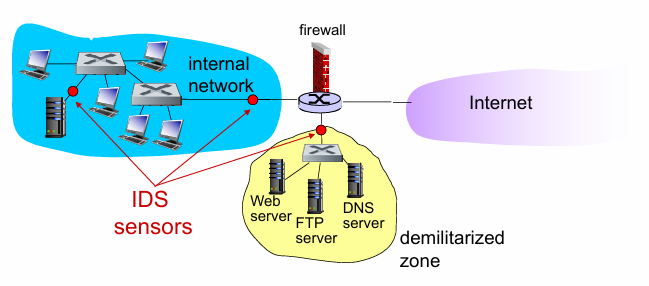
\includegraphics[width=0.9\linewidth]{immagini/firewall_3.png}
    \caption{\textbf{Mappa dei 3 sensori IDS.} I punti rossi indicano l'esatto posizionamento delle sonde: (1) nella \textit{DMZ}, per monitorare il traffico diretto ai server pubblici ; (2) al \textit{confine della rete interna}, per analizzare il traffico di interscambio LAN-Internet ; (3) nel \textit{cuore della rete interna}, per proteggere host e server locali dal traffico malevolo laterale .}
    \label{fig:posizionamento_ids}
\end{figure}

\newpage
\begin{notebox}{Posizionamento dei sensori IDS}
    
  \textbf{IDS in DMZ}
  
    Monitor del traffico diretto ai server pubblici (Web, FTP, DNS).
    Intercetta attacchi provenienti dall'esterno che hanno \emph{superato}
    il primo filtro del firewall.
    
    \vspace{0.6cm}
  \textbf{IDS nella rete interna}
  
    Rileva minacce generate da macchine interne gi\`a compromesse
    (\textit{insider threats}) o malware che si propagano lateralmente.

Con sensori multipli si ottiene una \textbf{visione stratificata} delle minacce:
nessun punto cieco nella topologia.
\end{notebox}


\begin{notebox}{Riepilogo: Firewall vs.\@ IDS}
\begin{center}
\begin{tabular}{lll}
\toprule
\textbf{Caratteristica} & \textbf{Firewall} & \textbf{IDS} \\
\midrule
Posizione nel flusso & Inline (blocca attivamente) & Passivo (copia del traffico) \\
Ispezione & Header L3/L4 & Payload completo (DPI) \\
Granularit\`a & Pacchetto singolo & Correlazione tra sessioni \\
Azione & Block / Allow & Alert / Log \\
Velocit\`a & Alta (regole semplici) & Bassa (analisi profonda) \\
Punto di forza & Blocca traffico non autorizzato & Rileva attacchi sofisticati \\
\bottomrule
\end{tabular}
\end{center}
\end{notebox}


\newpage

%%%%%%%%%%%%%%%%%%%%%%%%%%%%%%%%%%%%%%%%%%%%%%%%%%%%%%%%%%%%
\section{Riepilogo: Il Quadro Generale della Sicurezza}
%%%%%%%%%%%%%%%%%%%%%%%%%%%%%%%%%%%%%%%%%%%%%%%%%%%%%%%%%%%%

\begin{tcolorbox}[colback=blue!5!white, colframe=blue!75!black, title=\textbf{1. Gli Strumenti (Tecniche di base)}]
\begin{itemize}[leftmargin=*]
  \item \textbf{Crittografia (Confidenzialità):}
  \begin{itemize}
      \item \textit{Simmetrica:} Chiave condivisa, molto veloce (es. \textbf{AES}, DES).
      \item \textit{Asimmetrica:} Coppia di chiavi pubblica/privata, computazionalmente lenta (es. \textbf{RSA}).
      \item \textit{Ibrida:} Usa crittografia asimmetrica (es. RSA) solo per scambiare in modo sicuro una chiave di sessione simmetrica.
  \end{itemize}
  \item \textbf{Integrità e Non Ripudio:} Si calcola un'impronta fissa tramite funzioni di \textbf{Hash} (es. MD5). Cifrando l'Hash con la chiave privata del mittente si ottiene la \textbf{Firma Digitale}.
  \item \textbf{Autenticazione:} 
  
  \textbf{Nonce/Timestamp} per prevenire i \textit{Replay Attack}. 
  
  \textbf{CA} (Certification Authority) e \textbf{PKI} per certificare le chiavi pubbliche ed evitare attacchi \textit{Man-in-the-Middle}.
\end{itemize}
\end{tcolorbox}

\vspace{0.4cm}

\begin{notebox}{2. Implementazione ai vari livelli dello stack TCP/IP}
\vspace{0.2cm}
\renewcommand{\arraystretch}{1.4}
\small
\begin{tabularx}{\textwidth}{|l|l|X|}
\toprule
\textbf{Livello / Scenario} & \textbf{Protocolli} & \textbf{Meccanismi Chiave} \\
\midrule
\textbf{L7: Applicazione} \newline (E-mail Sicura) & PGP, \newline S/MIME & \textbf{Approccio Ibrido ("Pacchetto Completo"):} combina RSA per lo scambio sicuro della chiave di sessione e la Firma Digitale per garantire integrità e non ripudio. \\
\hline
\textbf{L4: Trasporto} \newline (Navigazione Web) & \textbf{SSL / TLS} & \textbf{SSL Handshake:} autenticazione tramite Certificati e negoziazione algoritmi. \textbf{Key Derivation:} generazione di 4 chiavi sessione distinte per direzione e funzione. \textbf{Record Protocol:} segmentazione del flusso con MAC e Numeri di Sequenza. \\
\hline
\textbf{L3: Rete} \newline (VPN) & \textbf{IPsec} & Protocolli \textbf{AH/ESP:}. \textbf{Modalità:} \textit{Tunnel} (incapsula l'intero pacchetto IP originale, ideale per VPN) o \textit{Transport}. Gestione automatica delle chiavi tramite \textbf{IKE}. \\
\hline
\textbf{L2: MAC / Wi-Fi} \newline (Wireless LAN) & WEP, \newline \textbf{WPA2} & \textbf{WEP:} obsoleto e vulnerabile a causa dell'IV a 24 bit trasmesso in chiaro e dell'uso di RC4. \textbf{WPA2 (802.11i):} standard robusto basato su AES-CCMP, autenticazione centralizzata (AS) e \textit{4-way handshake}. \\
\hline
\textbf{Sicurezza Operativa}  & \textbf{Firewall} \newline e \textbf{IDS} & \textbf{Firewall:} isolamento perimetrale tramite filtraggio header (\textit{Stateless/Stateful}) o Application Gateway (Proxy). 

\textbf{IDS:} analisi del payload tramite \textit{Deep Packet Inspection} (DPI) per rilevare firme di attacchi o anomalie. \\
\bottomrule
\end{tabularx}

\vspace{0.4cm}
\textbf{Note Integrative:}
\begin{itemize}
    \item \textbf{L'approccio Ibrido:} È la soluzione standard per bilanciare sicurezza e prestazioni, utilizzando la crittografia asimmetrica (più lenta) solo per proteggere la chiave simmetrica (più veloce) che cifrerà i dati reali.
    \item \textbf{Importanza dei Nonce:} Vengono utilizzati a vari livelli per prevenire i \textbf{Replay Attack}, garantendo che ogni sessione o messaggio scambiato sia unico e "fresco".
    \item \textbf{Certification Authority (CA):} È uno strumento indispensabile per evitare attacchi \textbf{Man-in-the-Middle} (MitM), in quanto valida in modo sicuro il legame tra una chiave pubblica e l'effettiva identità del suo titolare.
\end{itemize}
\end{notebox}


\end{document}